\chapter{Modelos y simulaciones númericas}

Este capítulo aborda el marco teórico previo y la metodología descrita para generar simulaciones de flujo de agua subterránea a partir de la ecuación de flujo. Las simulaciones se generaran a partir de la resolución del modelo que representa al fenómeno, donde se realizaran observaciones sobre el comportamiento del flujo y la utilidad de la implementación computacional. Cada conjunto de simulaciones corresponden a un caso en específico, donde se planteará el modelo conceptual, matemático y computacional para crear las simulaciones requeridas.

\section{Caso homógeneo}

El modelo que explica la dinámica del flujo en medios porosos es la ecuación diferencial descrita en la ecuación 1.48, su tratamiento se hará en forma bidimensional en los ejes x-y, en el caso de una vista en planta (ecuación \ref{eqn:mys1}), y sobre los ejes x-z en el caso de una vista en perfil (ecuación \ref{eqn:mys2}). El caso homogéneo es el más simple, ya que la función de conductividades hidráulicas adquieren un valor constante $K(x,y,z)=C$, por lo que la ecuación de flujo a resolver es similar a la ecuación 1.45 pero sin la componente y o z, dependiendo del plano donde obtendremos la solución del problema.

 \begin{equation}
 \label{eqn:mys1}
 \dfrac{\partial^{2}h}{\partial{x^{2}}}+\dfrac{\partial^{2}h}{\partial{y^{2}}}=0
\end{equation} 

 \begin{equation}
 \label{eqn:mys2}
 \dfrac{\partial^{2}h}{\partial{x^{2}}}+\dfrac{\partial{^{2}h}}{\partial{z^{2}}}=0
\end{equation} 

\subsection{Simulación 1: Condiciones de fronteras simples}

El modelo conceptual-teórico consiste en una porción de acuífero rectangular de 200 m en dirección E-O y 100 m en dirección N-S que se extiende sobre un plano de ladera con echado en dirección este. Las mediciones de la carga hidráulica indican valores de $h=100m$ en la frontera izquierda (Oeste) y $h=10m$ en la frontera derecha (Este), mientras que tanto la frontera superior (Norte) como la inferior (Sur) colindan con formaciones no permeables. El modelo conceptual para la vista en planta se puede ver representado en la figura 3.1. 

 \begin{figure}[H]
\centering
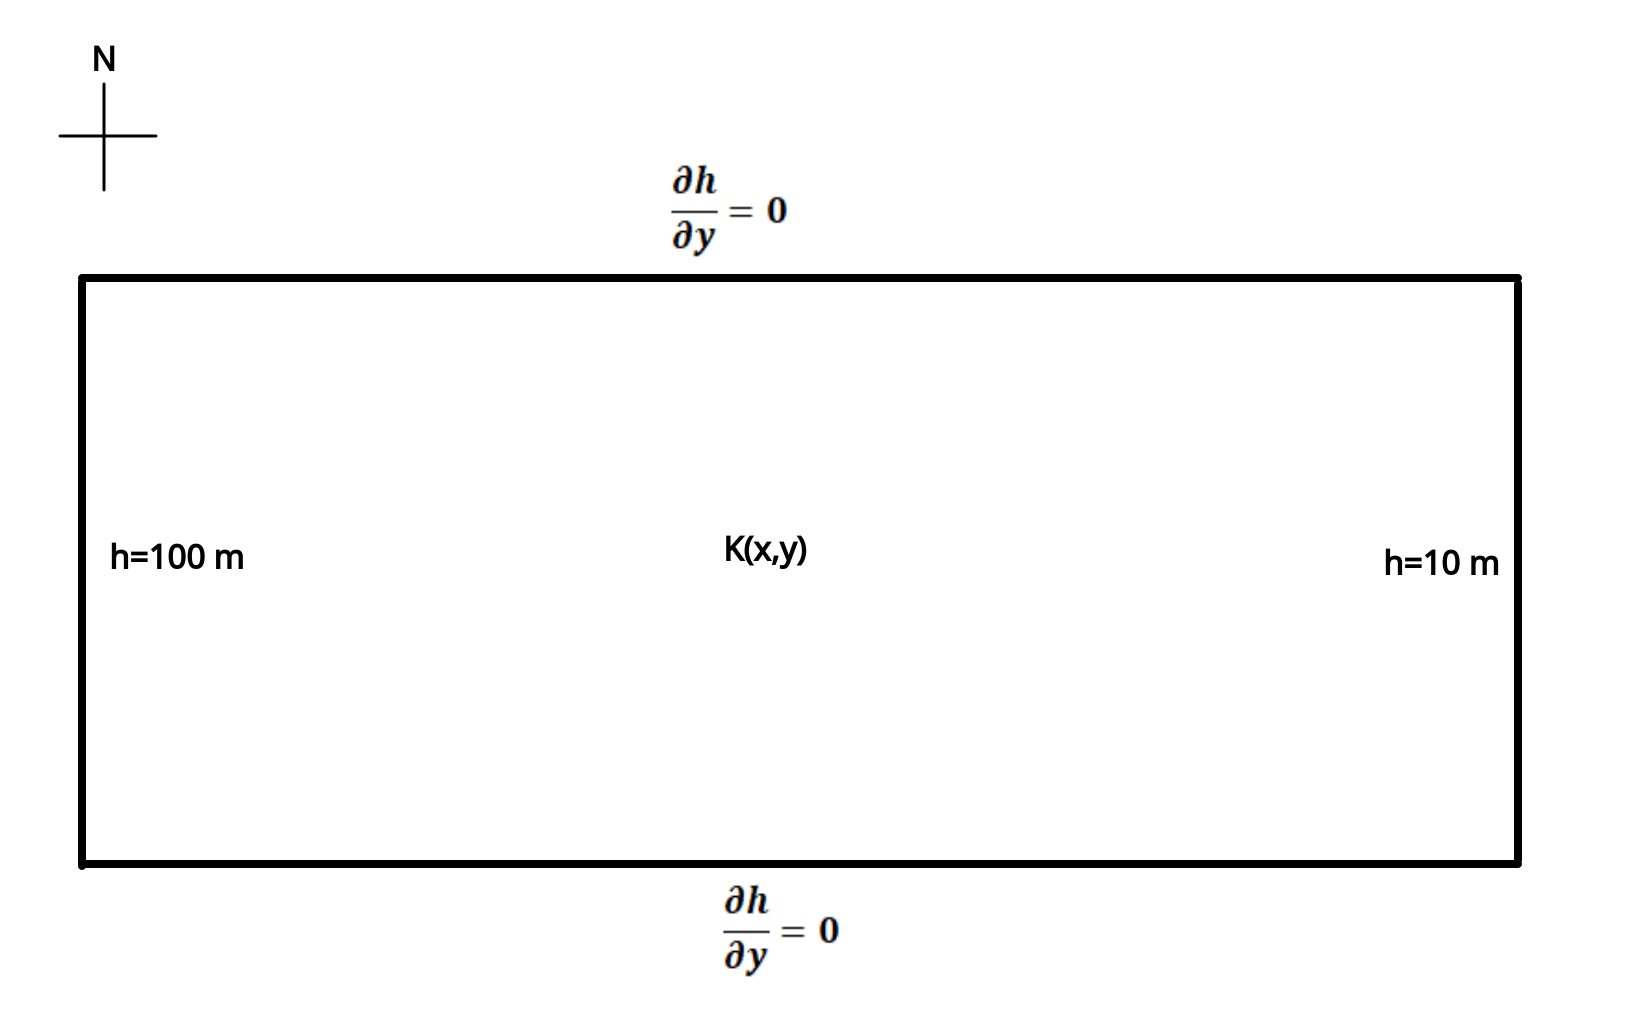
\includegraphics[scale=0.35]{Figura_25c.png}
\caption{ Modelo matemático y conceptual (Vista en planta)}
\label{Figura20:2}
\end{figure}

Para la vista en planta, el modelo matemático que representa al modelo conceptual es la ecuación \ref{eqn:mys1} , donde las condiciones de frontera son representadas por condiciones de Dirichlet en las fronteras Este-Oeste y condiciones de Neumann en las fronteras Norte-Sur.

 \begin{equation}
 \label{eqn:mys3}
 \nabla^{2}h(x,y)=0 \quad en \quad \Omega
\end{equation} 

\begin{equation}
 \label{eqn:mys4}
 h(x,y)=100 \quad en \quad {\partial}{\Omega}_{D1}
\end{equation}

\begin{equation}
 \label{eqn:mys4a}
 h(x,y)=10 \quad en \quad {\partial}{\Omega}_{D2}
\end{equation}
 
\begin{equation}
 \label{eqn:mys5}
  {\nabla}h{\cdot}\textbf{n}=0 \quad en \quad {\partial}{\Omega}_{N} 
\end{equation}  

Donde ${\nabla}^{2}h$ representa la ecuación \ref{eqn:mys1}; $\textbf{n}$ es el vector normal a la frontera ${\partial}\Omega$ y la frontera del problema se define como ${\partial}\Omega={\partial}\Omega_{D}{\cup}{\partial}\Omega_{N}$ y ${\partial}{\Omega}_{D}={\partial}\Omega_{D1}{\cup}{\partial}\Omega_{D2}$  . Según las caracteristicas del modelo conceptual, el domino y sus fronteras se plantean de la siguiente forma:

\begin{itemize}
\item  $\Omega=[0,100]{\times}[0,200]$ Dominio rectangular
\item  ${\partial}\Omega_{D}={(0,y){\cup}(200,y)}$ Condiciones de Dirichlet
\item  ${\partial}\Omega_{N}={(x,0){\cup}(x,100)}$ Condiciones de Neumann
\end{itemize}

La formulación integral de la ecuación \ref{eqn:mys3} se realiza a partir del método variacional, donde $v$ es nuestra función test correspondiente a nuestros espacio de Hilbert $H^{1}$, relajando las condiciones de derivabilidad al momento de multiplicar por nuestra función test y luego integrar, obtenemos la siguiente formulación integral expresada en su forma lineal y bilineal (veáse sección 2.2.1).

\begin{equation}
 \label{eqn:mys6}
 a(h,v)=\int_{\Omega}^{} {\nabla}h{\cdot}{\nabla}v \cdot ds
\end{equation}  

\begin{equation}
 \label{eqn:mys7}
 L(v)= \int_{\Omega}^{} fv \cdot ds + \int_{{\partial}_{N}}^{} {\nabla}h{\cdot}\textbf{n} \cdot ds
\end{equation}  

La segunda expresión de la ecuación \ref{eqn:mys7} son las condiciones naturales del problema variacional, asumiendo la condición dicha en la ecuación \ref{eqn:mys5}, este término se anula, además, el análisis de la porción del acuífero no contempla ningún tipo de fuentes o sumideros, por lo que la función $f$ es igual $0$, por lo que forma lineal queda $L(v)=0$.
\\

El espacio discreto de aproximación $\hat{H}^{1}$ de $H^{1}$, se construira a partir de elementos finitos triángulares del tipo galerkin continuo, con tres grados de libertad ($n(q)=3$), $\phi$ serán polinomios de grado 1 que sirven como base del espacio de funciones e imponiendo las condiciones de frontera esenciales del tipo dirichlet dentro del espacio $\hat{H}^{1}$. El espacio que discretiza nuestro problema es el siguiente.

\begin{equation}
\label{eqn:mys8}
\hat{H}^{1}=  \left[ \hat{h}(x,y) : \quad \displaystyle\sum_{j=1}^3  h_{j}\phi_{j}(x,y)  \quad  j=1,2,3, \quad h=100 \quad en  \quad {\partial}\Omega_{D1}, \quad h=10 \quad en \quad {\partial}\Omega_{D2} \right]     
\end{equation}  

El modelo númerico consiste en sustituir la solución $h(x,y)$ por el resultado discretizado a partir de las funciones de interpolación $\hat{h}(x,y)$ en sus grados de libertad, que se implementa de forma semiautomática a partir de las componentes de FeniCS: UFL y FFC, mientras que la construcción del espacio de funciones se realiza a través de la componente $FIAT$. 
\\

A partir del modelo matemático, la implementación computacional se realiza según lo planteado en la sección 2.3. Los resultados consisten en el campo de cargas hidráulicas en todo el dominio establecido (Vista en planta) y la descarga específica para cada elemento finito, donde la conductividad hidráulica es igual 1 en todo el dominio.
 \\

 \begin{figure}[H]
\centering
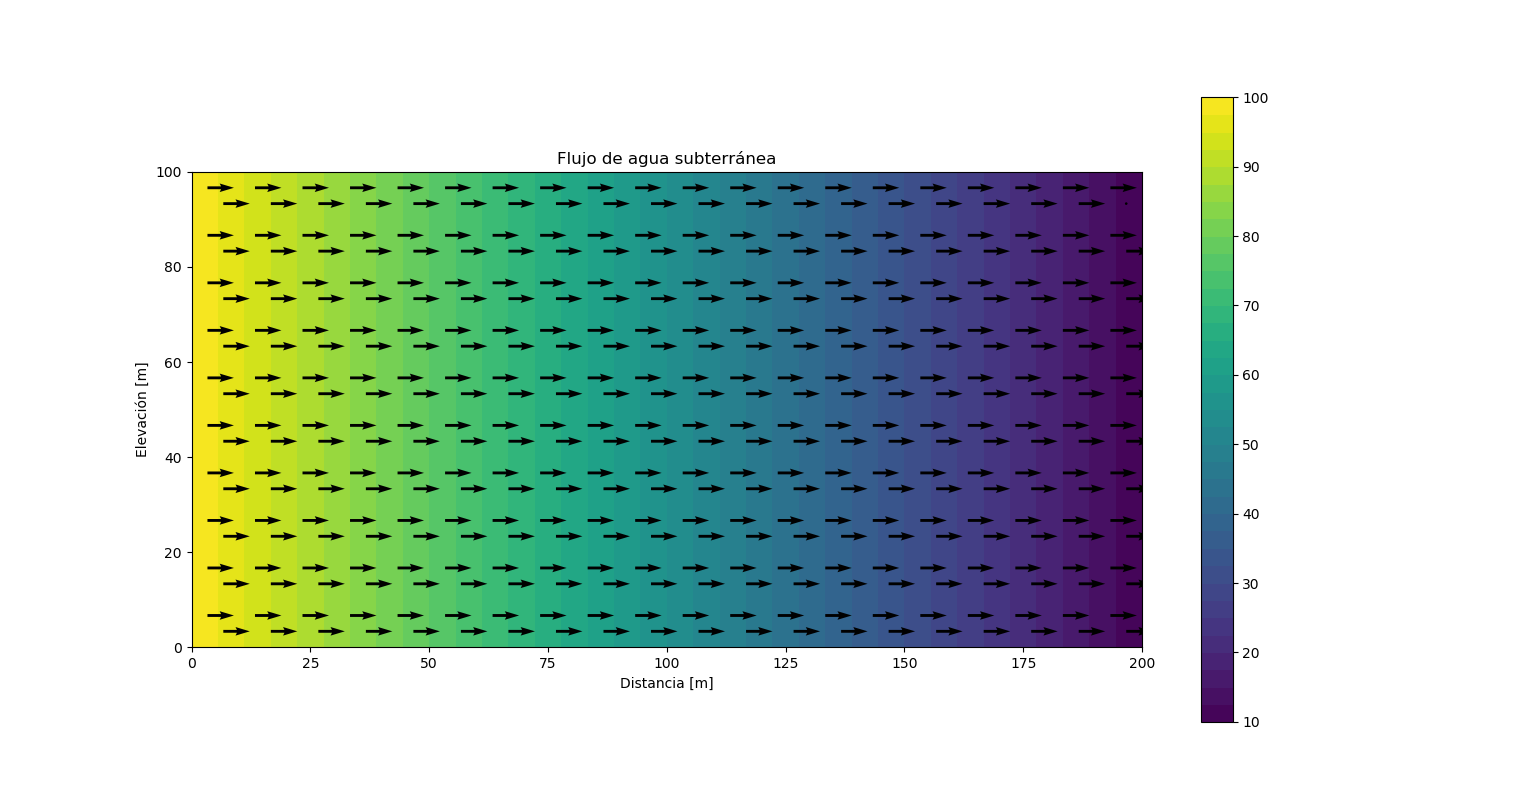
\includegraphics[scale=0.50]{Figura_26.png}
\caption{ Campo de cargas hidráulicas y flujo de agua subterránea (Vista en planta)}
\label{Figura20:2}
\end{figure}

Al ser un medio homogéneo, con valores constantes en las fronteras laterales y las fronteras superior e inferior impermeables, la teoría nos indica que el flujo se mueve de la zona de mayor carga hidráulica a la zona de menor carga hidráulica, debido a esto, el vector de descarga específica solo contiene componentes horizontales (dirección x), que es la dirección donde se mueve el flujo, de oeste a este. 
\\

Dado el caso de la vista en perfil, se realizará un corte del modelo anterior de oeste a este a una profundidad de 100m. La representación del modelo conceptual y matemática se observa en la figura \ref{Figura3:3}.

\begin{figure}[H]
\centering
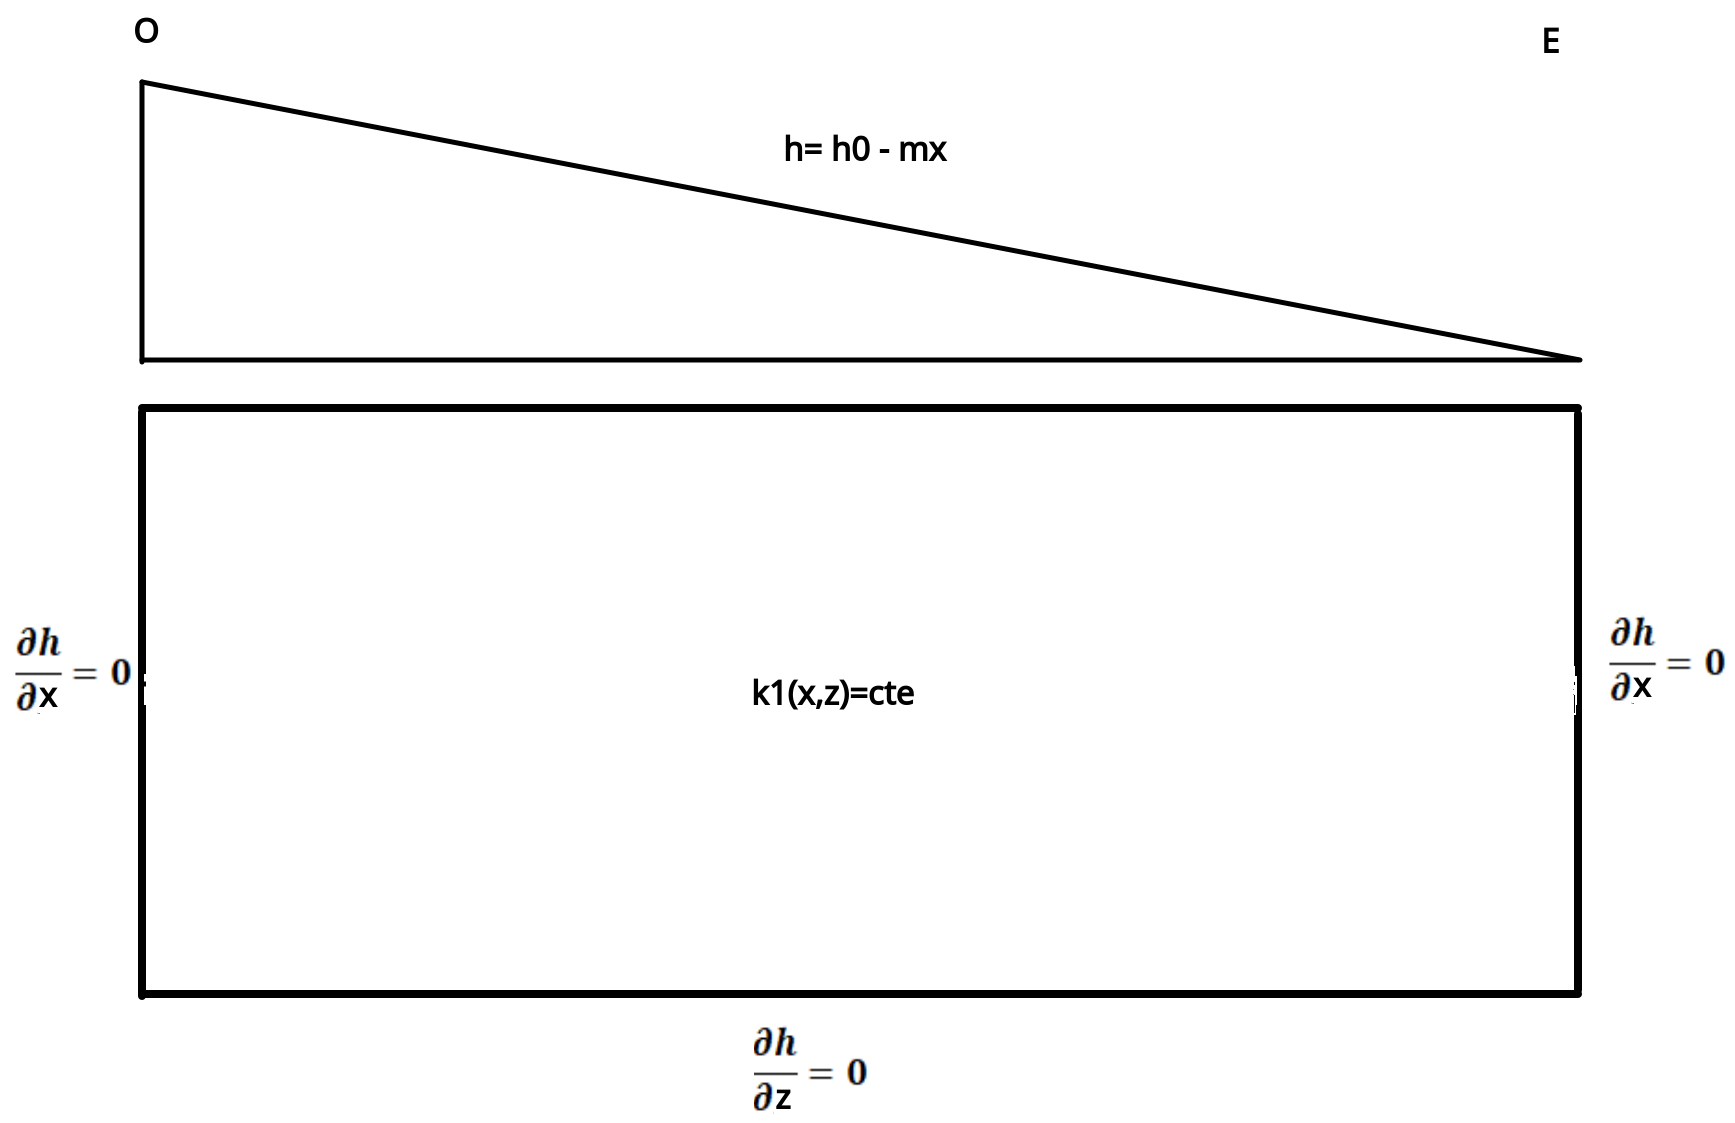
\includegraphics[scale=0.35]{Figura_27a.png}
\caption{ Modelo conceptual y matemático (Vista en perfil)}
\label{Figura3:3}
\end{figure}


La ecuación que modela este problema es la ecuación \ref{eqn:mys2}, donde la formulación integral y el espacio de funciones que discretiza nuestro problema es el mismo que el anterior (ecuación \ref{eqn:mys6} y ecuación \ref{eqn:mys8}). El cambio radica principalmente en la delimitación de las condiciones de frontera; las fronteras laterales y la frontera inferior se supondran barreras impermeables, mientras que la frontera superior se expresa como una función lineal donde la carga hidráulica varia en su valor máximo (100 m) hasta su valor minimo (10 m). Las condiciones de frontera para este problema son los siguientes:  

\begin{equation}
 \label{eqn:mys9}
    h=100-0.45x \quad en \quad {\partial}\Omega_{D}  
\end{equation}
 
\begin{equation}
 \label{eqn:mys10}
  {\nabla}h{\cdot}\textbf{n}=0 \quad en \quad {\partial}{\Omega}_{N} 
\end{equation}  

\begin{itemize}
\item  $\Omega=[0,200]{\times}[0,100]$ Dominio rectangular
\item  ${\partial}\Omega_{D}={(x,100)}$ Condiciones de Dirichlet
\item  ${\partial}\Omega_{N}={(x,0){\cup}(0,y){\cup}(200,y)}$ Condiciones de Neumann
\end{itemize}

A partir de estas nuevas condiciones de frontera, obtenemos el siguiente campo de cargas hidráulicas.

 \begin{figure}[H]
\centering
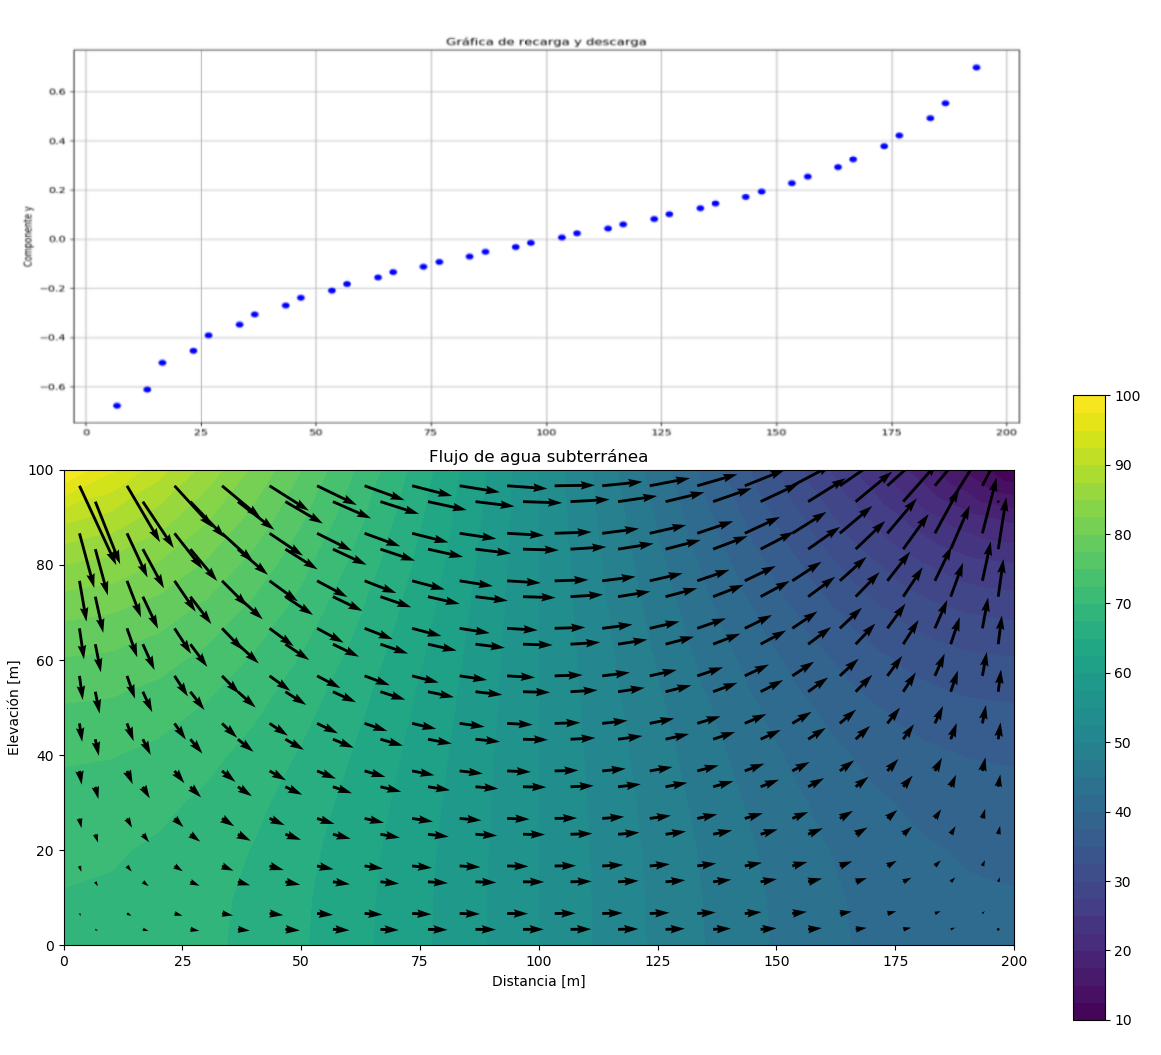
\includegraphics[scale=0.55]{Figure_28c.png}
\caption{Arriba, Gráfica de recarga y descarga; Abajo, Campo de cargas hidráulicas y flujo de agua subterránea (Vista en perfil)}
\label{Figura3:4}
\end{figure}

Según lo previsto de la sección en planta, las cargas hidráulicas decrecen de oeste a este, por lo que el flujo se mueve en esa dirección. Los valores del vector de descarga específica en este caso si tienen componentes tanto en dirección x como en dirección z, la componente en x se mantiene positiva en todo el modelo debido a que toma una dirección positiva de oeste a este, mientras que la componente en z se mantiene negativa hasta los 100 metros, donde la descarga específica solo tiene componente en x, para después de rebasar los 100 metros donde la componente se vuelve positiva e incrementa su valor conforme aumenta la distancia. Para observar mejor la zona de recarga y descarga, se elaboró una gráfica que muestra la variación de la componente z del vector de flujo en la superficie respecto a la distancia en x, siendo negativo la recarga y positivo la descarga, siendo nulo a la mitad de la distancia total.
\\

El anterior problema fue planteado de forma analítica por Josef Toth en 1962 para entender la forma en que se comportaba el flujo en pequeñas cuencas de drenaje. La ecuación que define el campo de carga hidráulica para el problema anterior, se define de la siguiente forma (Toth,1962):

\begin{equation}
 \label{eqn:mys10.1}
  h= (z_{0}+\dfrac{cs}{2})-\dfrac{4cs}{{\pi}^{2}}{\sum_{m=0}^{\infty}\dfrac{cos[(2m+1){\pi}x/s]cosh[2m+1]{\pi}z/s}{(2m+1)^{2}cosh[(2m+1){\pi}z_{0}/s]}} 
\end{equation}  
\\

Donde en la ecuación \ref{eqn:mys10.1}, $z_{0}$ es la condición de frontera izquierda igual a $100 m$; $s$ es la longitud de la cuenca, que en esta simulación es $s= 200 m$; $c$ es la pendiente de la ecuación que define la condición de Dirichlet en la parte superior de la cuenca ($45^{\circ}$); $x$ y $z$ son las coordenadas donde se requiere encontrar la carga hidráulica $h$; mientras que $m$ es una constante en una sumatoria que mientras tienda a $\infty$ obtendremos la solución completa. El campo de cargas hidráulicas para las condiciones anteriormente establecidas y con $m=200$ se graficó y se comparó con la solución obtenida a partir del método de elemento finito con FEniCS, obteniendo el siguiente mapa de error absoluto.

 \begin{figure}[H]
\centering
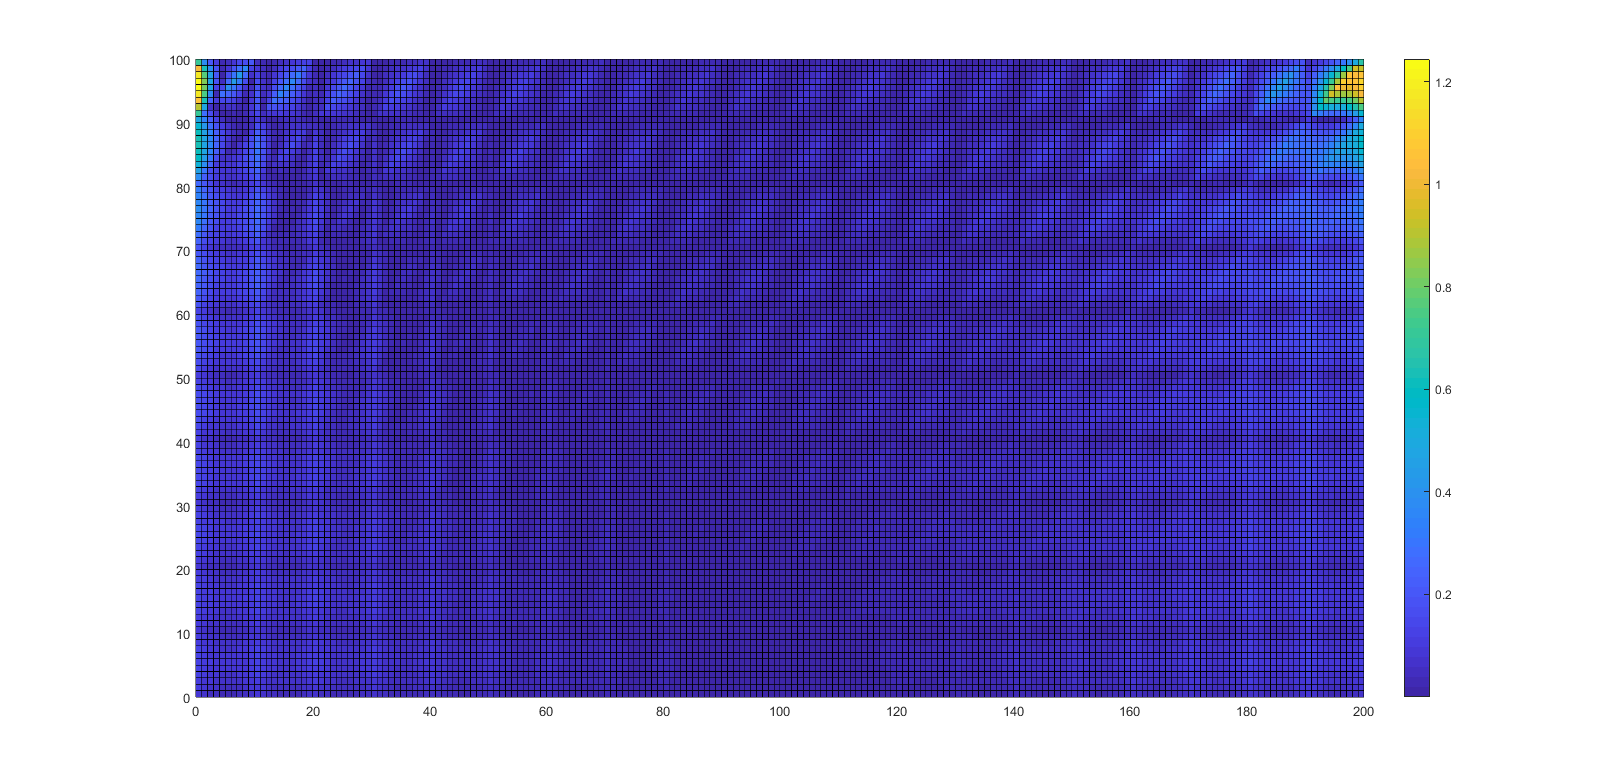
\includegraphics[scale=0.40]{Figura_28.5.png}
\caption{Mapa de error absoluto en el dominio; solución con FeniCS vs solución analitica de Toth (m=200)}
\label{Figura3:4.5}
\end{figure}

En la figura \ref{Figura3:4.5} podemos observar como el error es minimo en la mayor parte del dominio, especialmente en el centro, siendo los extremos de las fronteras que fueron definidas por las condiciones de Dirichlet, las zonas de mayor error, esto se debe a que la solución analitica de Toth se evaluó con una sumatoria $m=200$ que mantiene cierto error al no poder evaluarse con $m$ tendiendo al infinito. De esta forma, se valida la solución obtenida con FEniCS y  
se nota la ventaja del método de elemento finito al mantener  los valores de la condicion de Dirichlet de la forma en que se definieron en un principio.  

\subsection{Simulación 2: Condiciones de fronteras complejas}

Las condiciones de frontera se pueden complicar para aproximarse a condiciones más exactas a la realidad. Siguiendo el caso del modelo anterior, el flujo viaja de este a oeste para una carga hidráulica descendiente, sin embargo, el movimiento del flujo cambia dependiendo de la geometría de frontera, donde usualmente la forma de la carga hidráulica en la superficie recrea su topografía.
\\

Para la siguiente simulación se recrearon las condiciones de la misma forma que en la simulación anterior, cambiando la condición de frontera superior para obtener una mayor aproximación a un caso real, en este caso se simuló el perfil topográfico de un valle intermontano, cuyas laderas se extienden en el lado izquierdo de 0 a 40 metros con un valor de carga hidrálica inicial $h=500 m$, el valle se encuentra de 40 a 160 metros con un valor de carga hidráulica al ras del valle intermontano $h=100 m$, y una ladera correspondiente a otra montaña que colinda de 160 a 200 metros con $h=500 m$ en el extremo de la ladera. Para obtener un mayor acercamiento a la realidad, tanto las laderas como el valle tendrán una variación senoidal simulando la irregularidad del subsuelo. El modelo conceptual se muestra en la figura \ref{Figura3:3a}, donde las conductividades $K1$ y $K2$ son iguales para el caso homogéneo. 

 \begin{figure}[H]
\centering
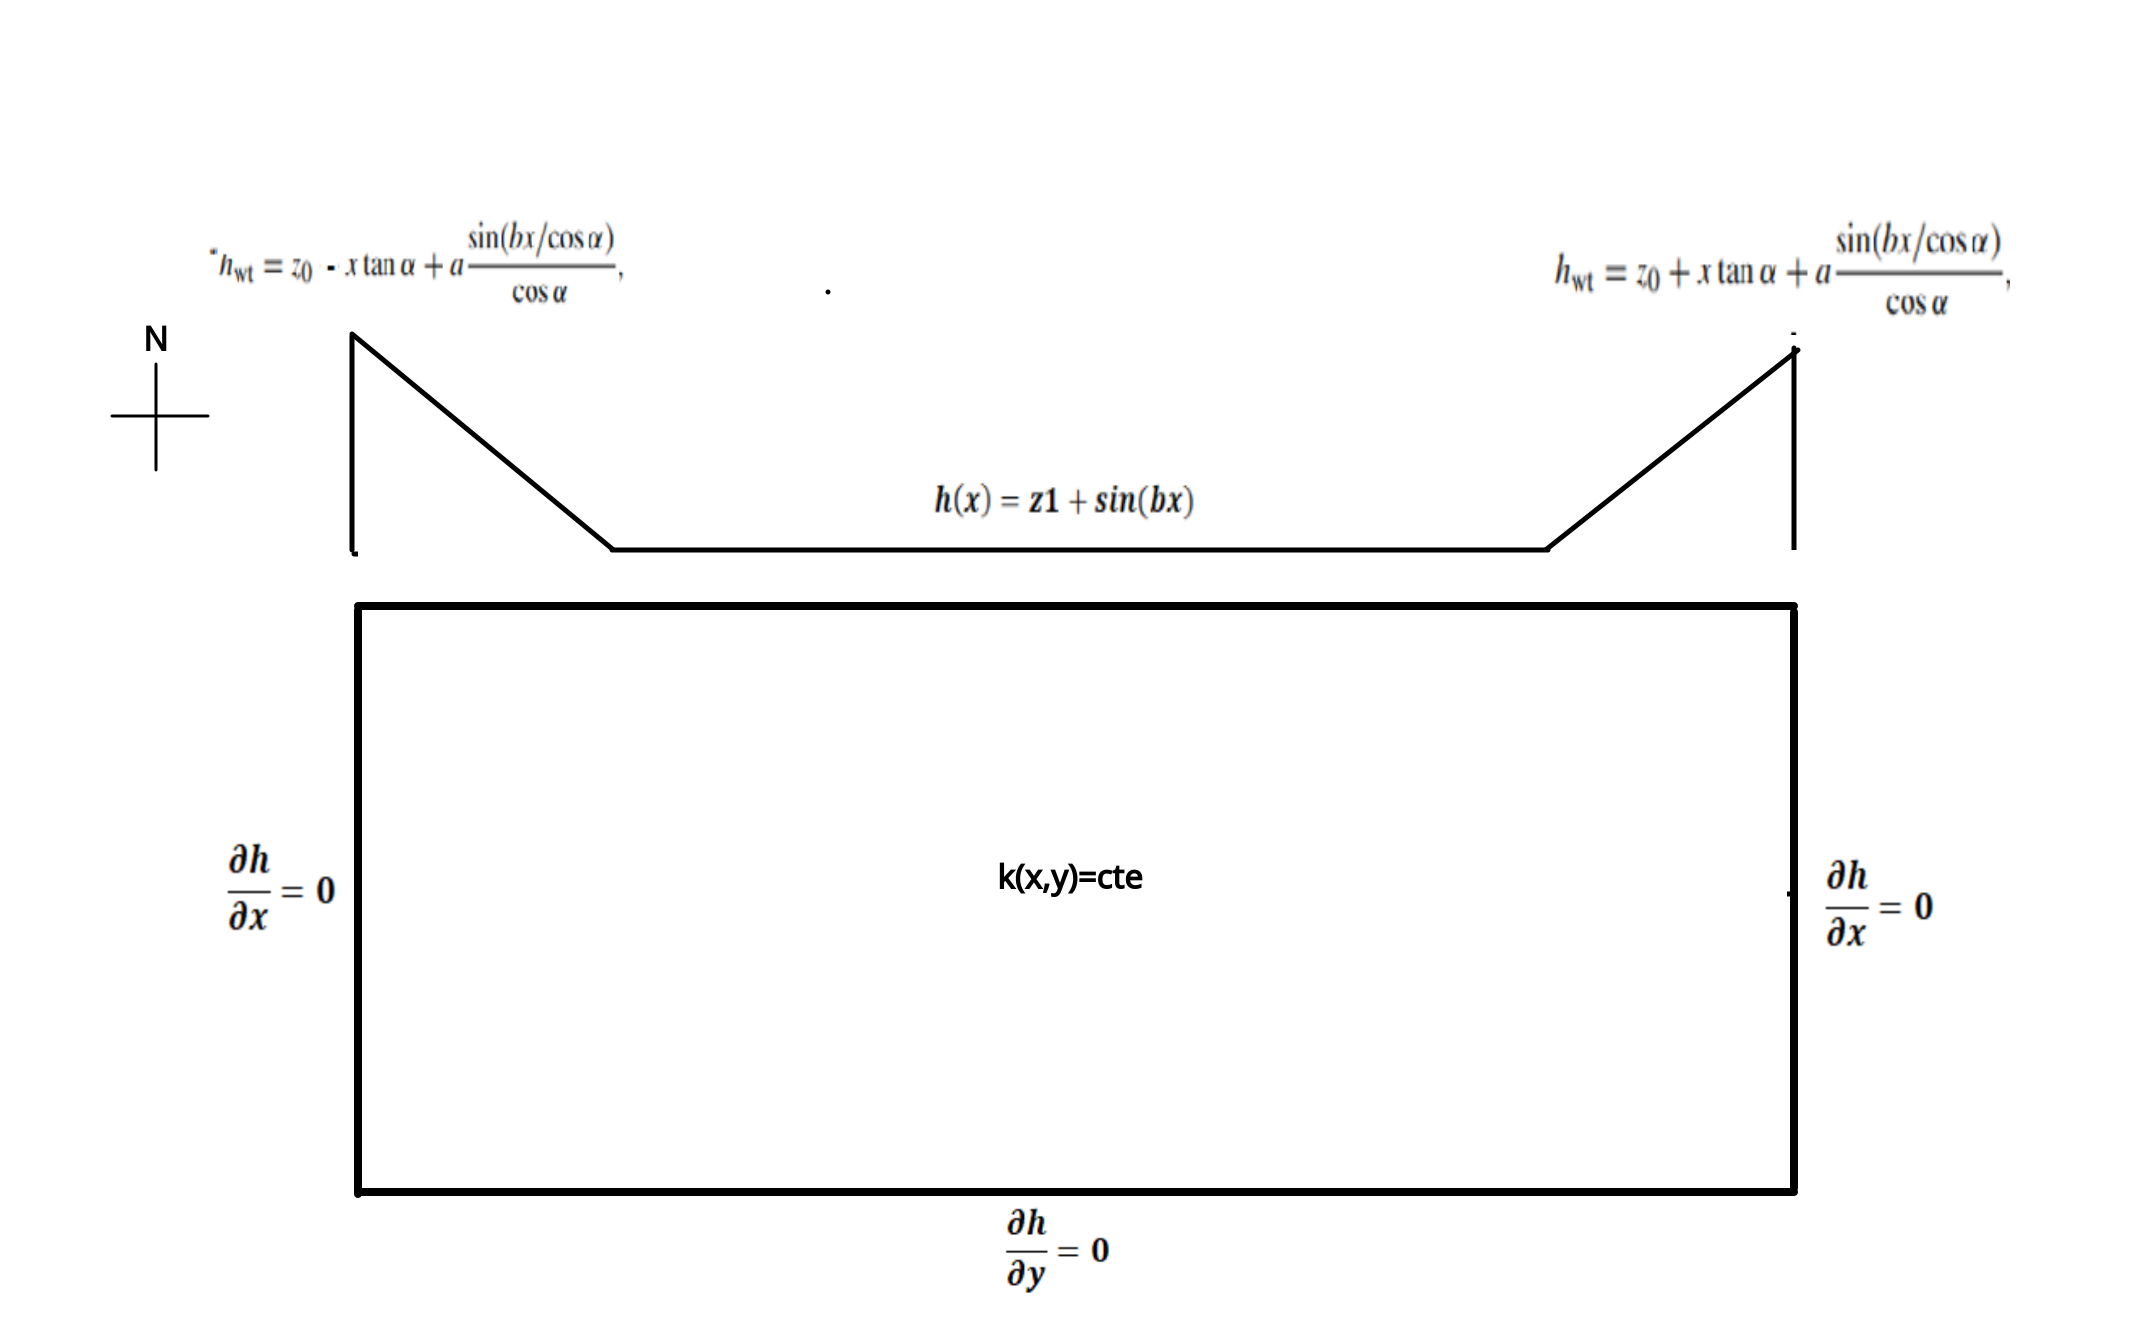
\includegraphics[scale=0.30]{Figura_29c.png}
\caption{ Modelo conceptual y matemático}
\label{Figura3:3a}
\end{figure}

El modelo matemático es el mismo que en la ecuación \ref{eqn:mys8}, con las mismas condiciones de Neumann (ecuación \ref{eqn:mys10}), pero variando en las condiciones de frontera de Dirichlet (ecuación \ref{eqn:mys9}) de la siguiente forma:

\begin{itemize}
\item  ${\partial}\Omega_{D_{Izquierda}}={([0,40],100)}$
\item  ${\partial}\Omega_{D_{Central}}={([40,160],100)}$
\item  ${\partial}\Omega_{D_{Derecha}}={([160,200],100)}$ 
\end{itemize}

 \begin{equation}
 \label{eqn:mys11}
    h=500-x{\cdot}tan(1.4711)+(\dfrac{cos(1000{\cdot}x/cos(1.4711) }{cos(1.4711)}) \quad en \quad  {\partial}\Omega_{D_{Izquierda}}    
    \end{equation}

\begin{equation}
 \label{eqn:mys12}
    h= 100+10{\cdot}(sin(1000{\cdot}x)) \quad  en \quad {\partial}\Omega_{D_{Central}}
\end{equation}

\begin{equation}
 \label{eqn:mys13}
    h= -1500+x{\cdot}tan(1.4711)+(\dfrac{cos(1000{\cdot}x/cos(1.4711) }{cos(1.4711)}) \quad en \quad  {\partial}\Omega_{D_{Izquierda}}   
\end{equation}

A partir de estas condiciones de Dirichlet y aplicando la metodología para la simulación de flujo, obtenemos los siguientes resultados:

 \begin{figure}[H]
\centering
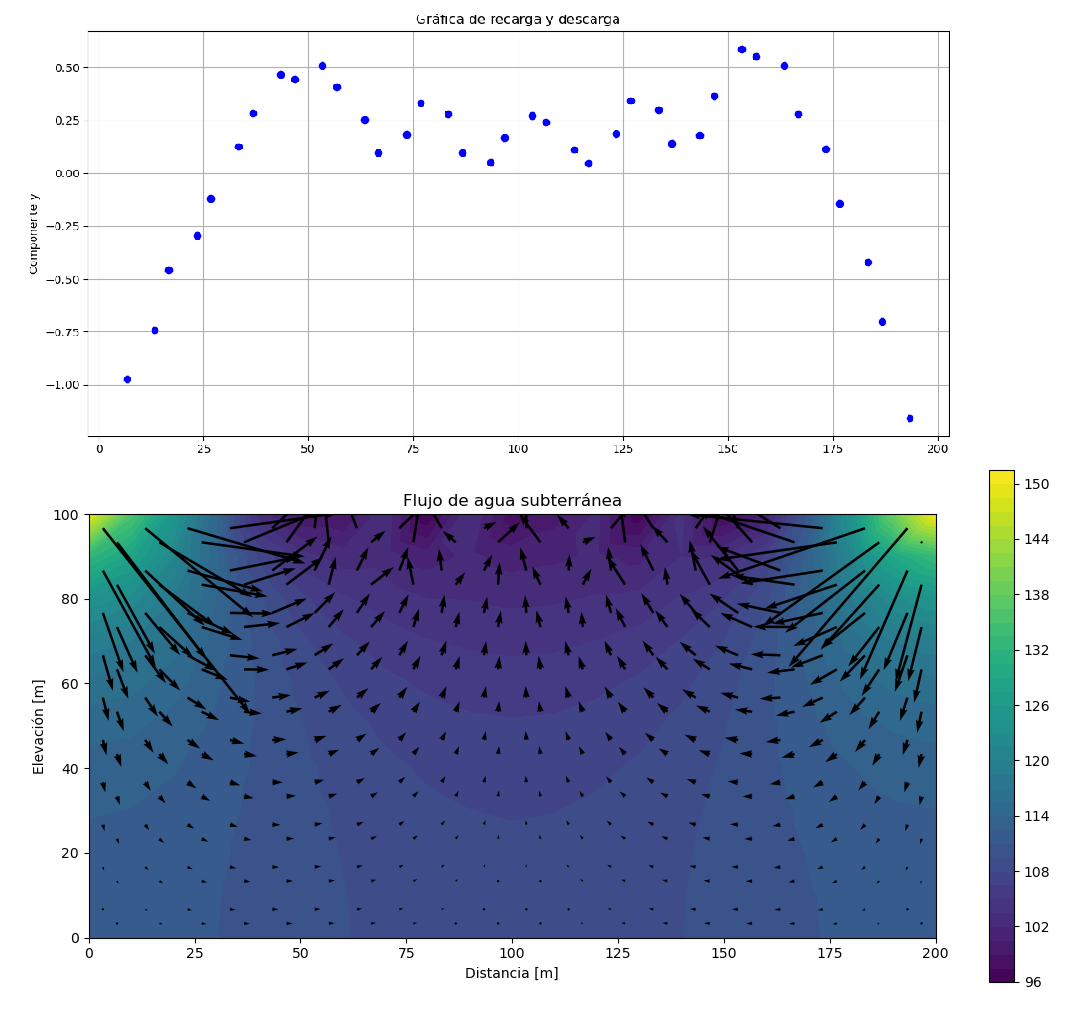
\includegraphics[scale=0.55]{Figura_29e.png}
\caption{ Campo de cargas hidráulicas y flujo de agua subterránea (Vista en perfil)}
\label{Figura20:2}
\end{figure}

Con esta simulación podemos observar que las cargas hidráulicas tienen un valor máximo en los extremos y disminuyen conforme nos vamos acercando al centro del valle. Esta simulación es importante debido a que nos muestra la importancia de entender la topografía de nuestro modelo, pues una simulación de vista en planta con valores de frontera de Dirichlet constantes y fronteras impermeables, nos daria una simulación de cargas hidráulicas constantes sin movimiento de flujo en todo el dominio, cuando en realidad el flujo se concentra en la zona central que corresponde al área del valle intermontano.
\\

El análisis de la componente z en la superficie indica como el flujo funciona como recarga en las zonas más altas, donde su valor disminuye hasta convertirse en descarga, alcanzando su punto máximo a principios del valle, posteriormente la descarga disminuye sobre el centro del valle y alcanza su máximo en el otro extremo del valle, volviendo a ser la zona montañosa el área de recarga, en esta gráfica se puede apreciar mejor la influencia de la variación senoidal, afectando principalmente la descarga en el centro del valle.

\section{Caso heterogéneo simple}

La ecuación que modela este tipo de caso es similar al anterior, solo que la conductividad hidráulica $K(x,y,z)$ tendrá diferente valor dependiendo de la zona del dominio en el que se encuentre. La asignación de la heterogeneidad se hará dependiendo del modelo conceptual que se trabaje; las ecuaciones que modelan estos casos son los siguientes:

\begin{equation}
\label{eqn:phi14}                         
\dfrac{\partial}{\partial{x}}(K(x,y)\dfrac{\partial{h}}{\partial{x}})+\dfrac{\partial}{\partial{y}}(K(x,y)\dfrac{\partial{h}}{\partial{y}})=0
\end{equation}

\begin{equation}
\label{eqn:phi15}                         
\dfrac{\partial}{\partial{x}}(K(x,z)\dfrac{\partial{h}}{\partial{x}})+\dfrac{\partial}{\partial{z}}(K(x,z)\dfrac{\partial{h}}{\partial{z}})=0
\end{equation}

\subsection{Simulación 3: Condiciones de fronteras simples}

El modelo conceptual-teórico consiste en el mismo modelo de la simulación 1 (sección 3.2), donde vamos a definir  una sección con diferente material. La asignación de la conductividad hidráulica que caracteriza al material se realiza con base en los resultados presentados por De Marsily (1986) (Figura 1.2). En este caso se tomará en cuenta dos modelos donde el medio geológico corresponde a un cambio de facies de un material de grano grueso, de valor promedio $K=100 m/d{\acute{i}}a$ a un material de grano más fino con valor promedio $K=10 m/d{\acute{i}}a$, y el otro modelo donde el cambio va de un material fino a un material más grueso. El cambio de facies se hace a partir de una linea diagonal en dirección Este-Oeste, a partir de estos valores construimos la ecuación que representa la conductividad hidráulica en todo el dominio de la siguiente forma:

\begin{equation}
 \label{eqn:mys16}
    k(x,y)= \left\{ \begin{array}{lcc}
             100 &   en  & {\Omega}_{1} \\
             \\ 10 &  en & {\Omega}_{2} \\
             
             \end{array}
   \right.
\end{equation}

Para el caso contrario se invierten los valores de conductividad hidráulica, además, la ecuación \ref{eqn:mys16} representa la distribución de la conductividad tanto para la vista en planta como en la vista en perfil.
\\

Las condiciones de frontera que se ocupan son las mismas que en la ecuación \ref{eqn:mys4}, \ref{eqn:mys4a} y \ref{eqn:mys5}; mientras que la ecuación que modela el problema es la siguiente:

\begin{equation}
 \label{eqn:mys17}
 {\nabla}k(x,y){\nabla}h(x,y)=0 \quad en \quad \Omega
\end{equation} 

La formulación integral se plantea a partir de la división del dominio $\Omega$ en subdominios con su propia conductividad hidráulica. Los subdominios y las fronteras del dominio quedan definidos de la siguiente manera:

\begin{itemize}
\item  ${\Omega}_{1}=[0,100]{\times}[0,100]$ Subdominio 1
\item  ${\Omega}_{2}=[100,200]{\times}[0,100]$ Subdominio 2
\item  ${\partial}\Omega_{D}={(0,y){\cup}(200,y)}$ Condiciones de Dirichlet
\item  ${\partial}\Omega_{N}={(x,0){\cup}(x,100)}$ Condiciones de Neumann
\end{itemize}

La formulación integral del problema se obtiene sobre los dos subdominios, obteniendo la siguiente forma bilineal:

\begin{equation}
 \label{eqn:mys18}
 a(h,v)=\int_{\Omega_{1}}^{} k_{1}{\nabla}h{\cdot}{\nabla}v \cdot ds+\int_{\Omega_{2}}^{} k_{2}{\nabla}h{\cdot}{\nabla}v \cdot ds
\end{equation} 

Mientras que la forma lineal de la formulación integral del problema al tener las mismas condiciones de fronteras es $L(v)=0$. La discretización del problema se realiza con el espacio de funciones planteado en la ecuación \ref{eqn:mys8} tanto para la vista en planta como para la vista en perfil; la simulación en planta para un cambio de facies de grano grueso a grano fino se observa en la figura \ref{Figura3:5}, mientras que el cambio de una facies de grano fino a grueso se observa en la figura \ref{Figura3:6}

\begin{figure}[H]
\centering
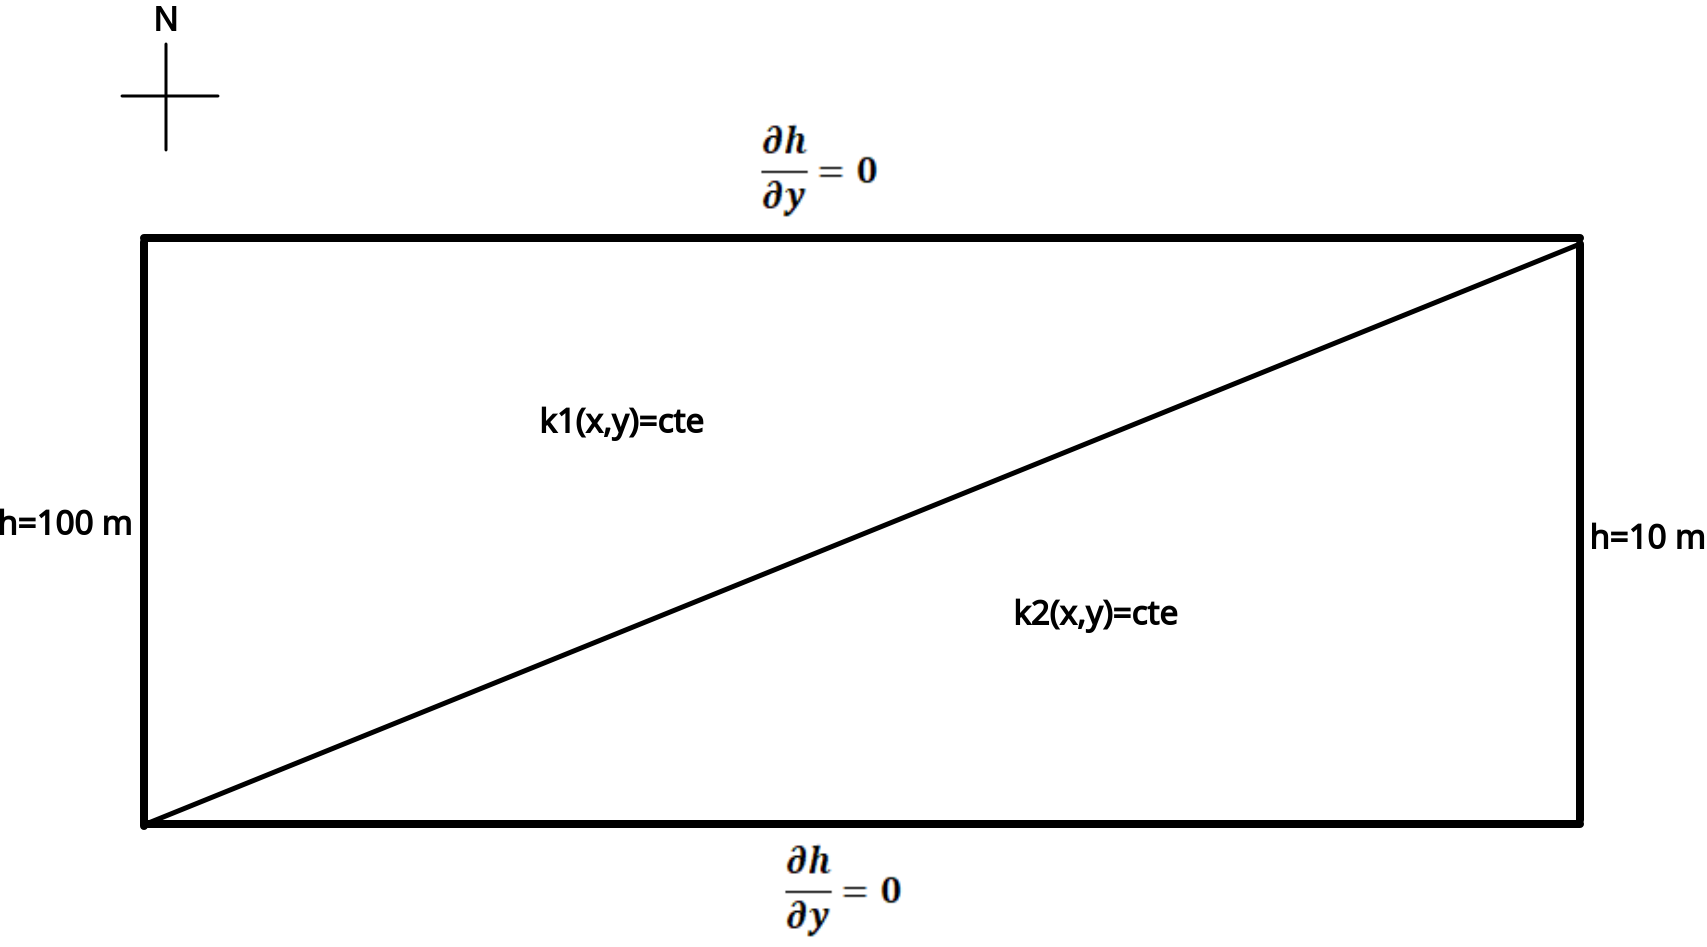
\includegraphics[scale=0.27]{Figura_25d.png}
\caption{ Modelo matemático y conceptual}
\label{Figura3:7a}
\end{figure}

 \begin{figure}[H]
\centering
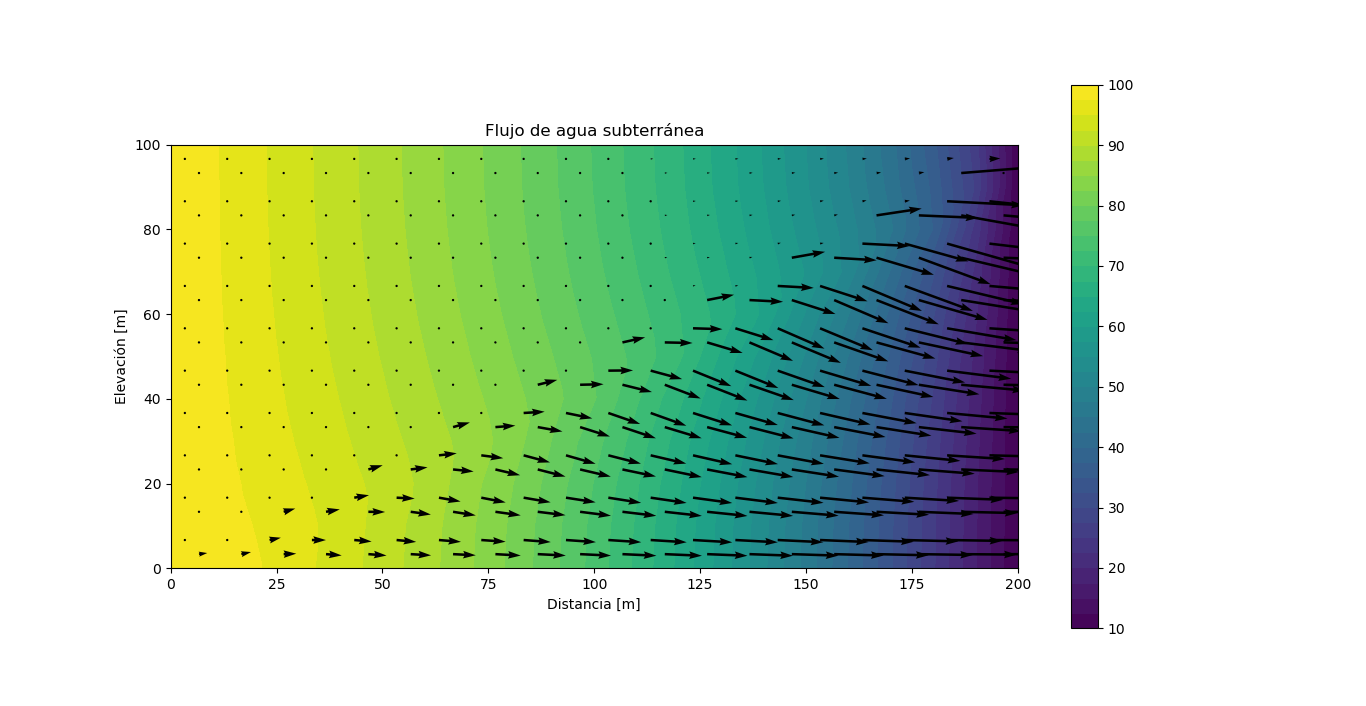
\includegraphics[scale=0.55]{Figura_31.png}
\caption{ Cambio de facies de grano fino a grueso}
\label{Figura3:5}
\end{figure}

 \begin{figure}[H]
\centering
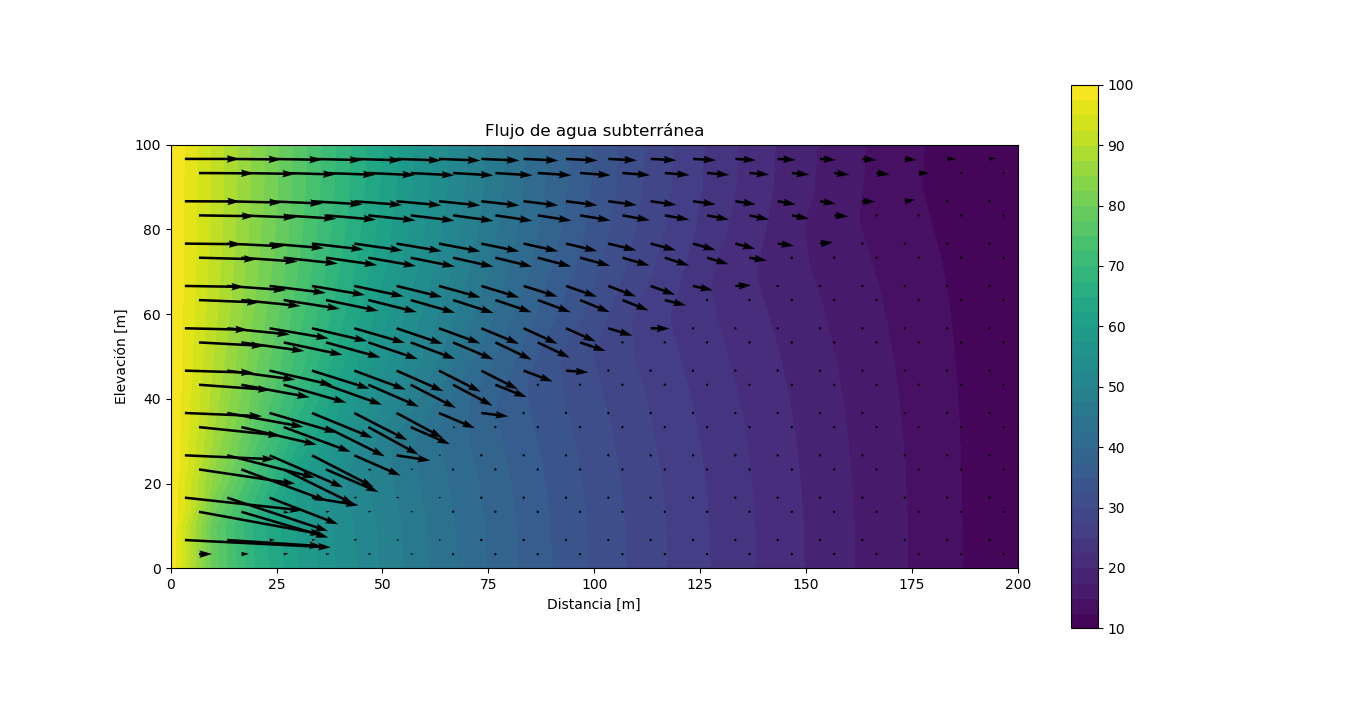
\includegraphics[scale=0.55]{Figura_32.png}
\caption{ Cambio de facies de grano grueso a fino}
\label{Figura3:6}
\end{figure}

A partir de los resultados anteriores, podemos observar en la figura \ref{Figura3:5} que el cambio de facies provoca que las isolineas de cargas hidráulicas se expandan en la zona de baja conductividad hidráulica, mientras que las isolíneas en las zonas de alta conductividad hidráulica se contraen, esto indica que la descarga específica tiene un  valor pequeño respecto a la zona de alta conductividad. Lo anterior se ejemplifica en la longitud de las flechas, donde se observa la dificultad del movimiento del flujo hasta la zona de transición, donde gradualmente aumenta el valor del flujo hasta el extremo del modelo; además, estas simulaciones nos comprueban la validez de ley tangente, al cambiar la dirección del flujo al momento de pasar a un estrato de diferente composición.
\\

Como en el caso homogéneo, la vista en perfil nos permite tener una visión más clara del movimiento del flujo  en el subsuelo, y en conjunto con la vista en planta, nos ayuda a tener un mejor panorama de la dirección y sentido del flujo. La simulación de la vista en perfil tendrá las mismas características que la homogénea, solo que en esta ocasión en el modelo teórico-conceptual los subdominios con diferente condutividad se encuentran a profundidad, en este caso representan dos estratos con diferente conductividad hidráulica que corresponden a un sedimento de grano fino y un sedimento de grano grueso. La ecuación que representa la conductividad hidráulica es igual a la ecuación \ref{eqn:mys16}, donde los subdominios ${\Omega}_{1}$ y ${\Omega}_{2}$ son los siguientes:

\begin{itemize}
\item  ${\Omega}_{1}=[0,200]{\times}[0,100]$ Subdominio 1
\item  ${\Omega}_{2}=[0,200]{\times}[100,200]$ Subdominio 2
\end{itemize}

El espacio de funciones que discretizan el dominio en elementos finitos y las condiciones de frontera seran iguales que en el caso homogéneo. Los resultados para este planteamiento de la heterogeneidad son las siguientes:

\
\begin{figure}[H]
\centering
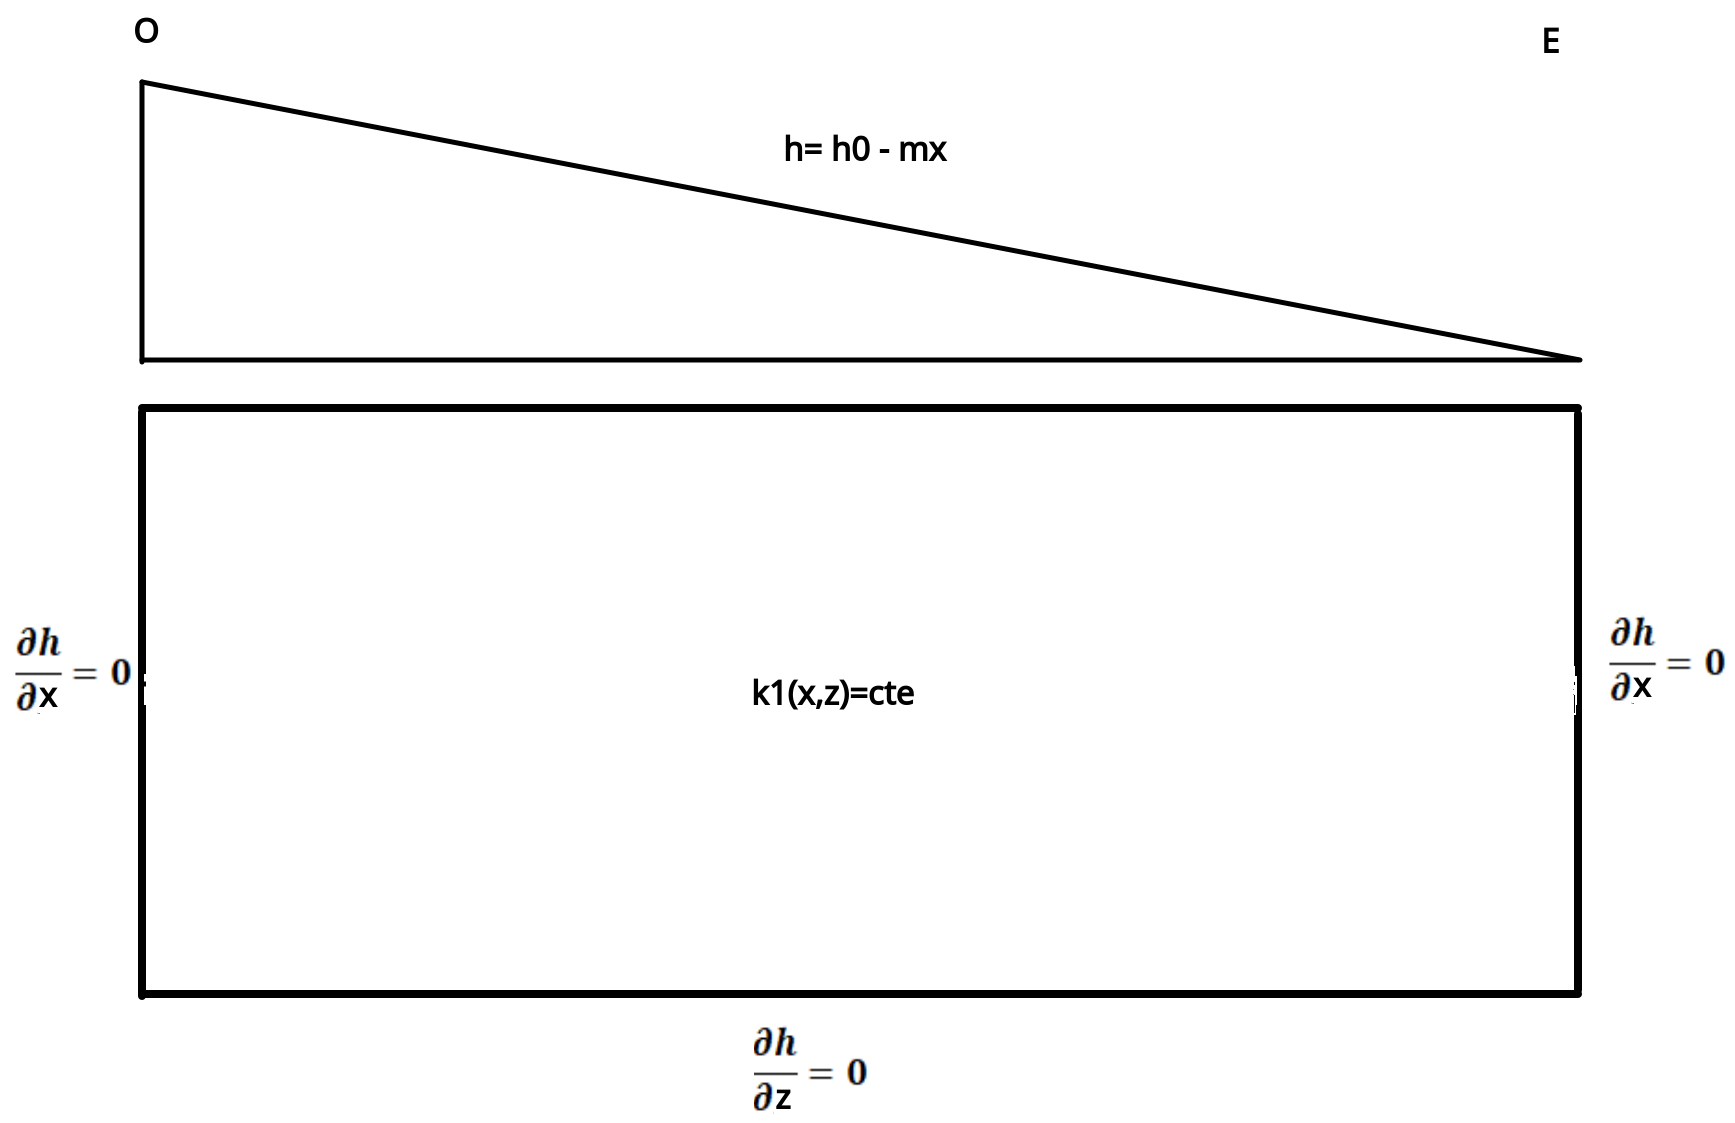
\includegraphics[scale=0.25]{Figura_27a.png}
\caption{ Modelo matemático y conceptual}
\label{Figura3:7a}
\end{figure}

\newpage

 \begin{figure}[H]
\centering
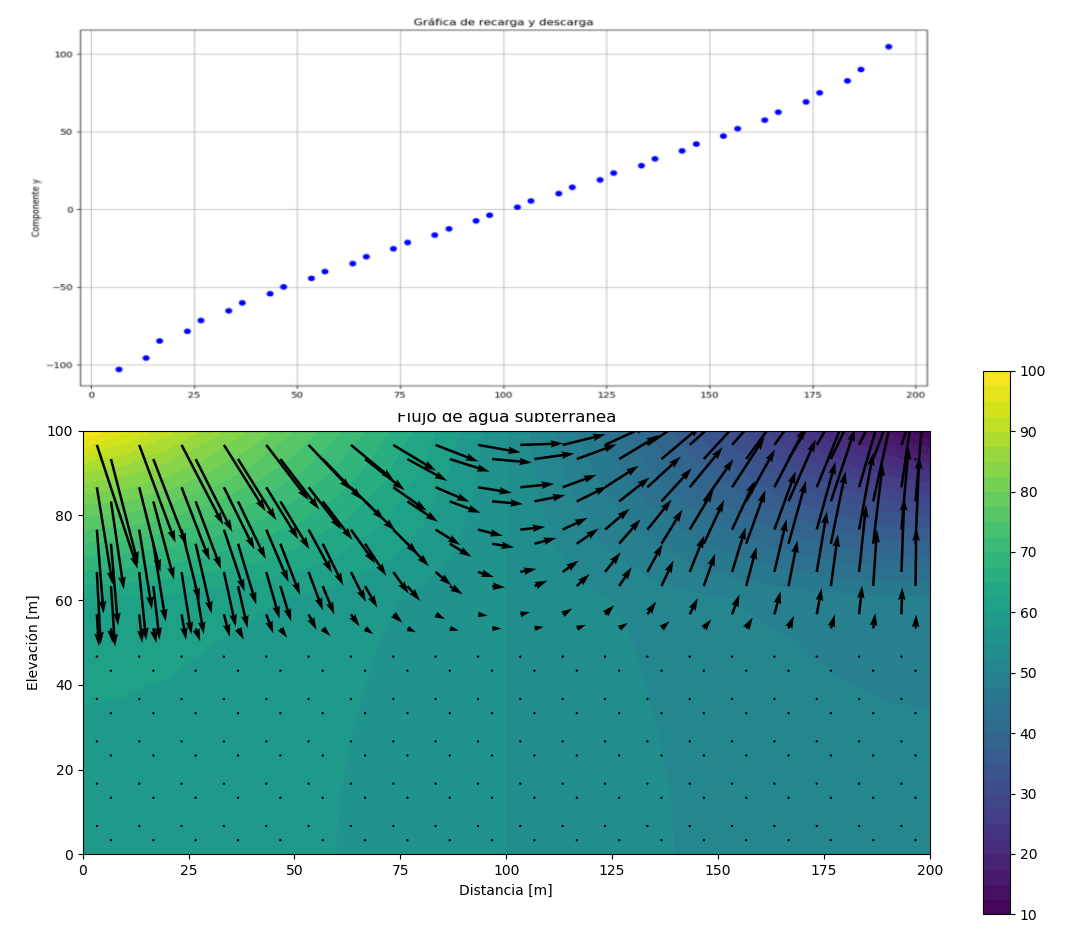
\includegraphics[scale=0.57]{Figura_33e.png}
\caption{ Estratificación grano grueso a fino}
\label{Figura3:7c}
\end{figure}

\begin{figure}[H]
\centering
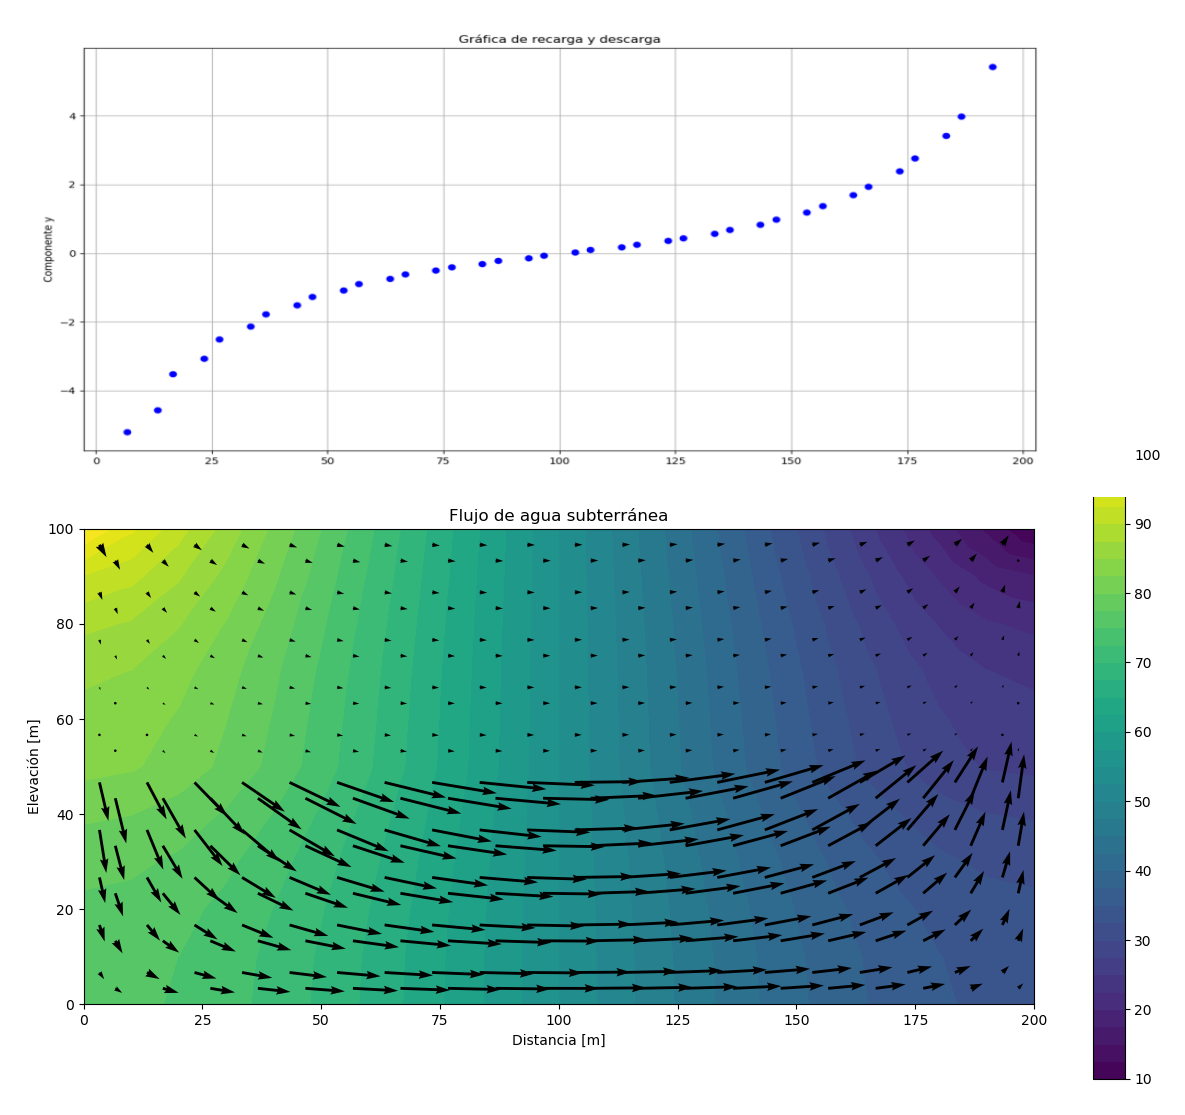
\includegraphics[scale=0.55]{Figura_34d.png}
\caption{ Estratificación grano fino a grueso}
\label{Figura3:7b}
\end{figure}


En este caso, en la figura \ref{Figura3:7c} se puede observar que la zona superior de alta conductividad, tiene un parecido al campo de cargas hidráulicas en un material homogéneo, sin embargo, en la zona de transición el flujo disminuye y se vuelve casi vertical con magnitudes muy pequeñas debido a la oposición que ofrece el material al paso del agua, una particularidad de esta simulación es que las lineas de flujo en la superficie convergen a una distancia más corta, por lo que las zonas de flujo local, intermedio y regional son más evidentes.
\\

En el caso de la figura \ref{Figura3:7b} las zonas de flujo  se amplian, mostrando una mayor distancia de recorrido antes de converger en la superficie, una observación importante de esta simulación es que el flujo es más rápido en la superficie y converge tanto en magnitud como en dirección en las zonas más profundas y cercanas al basamento (frontera impermeable), la anterior observación se comprueba al hacer la comparación con la figura  \ref{Figura3:4} correspondiente a la simulación de material homogéneo. 
\\

En el caso del material homogéneo, la magnitud y la dirección del flujo alcanza gradualmente un equilibrio hasta el basamento, mientras que en la figura \ref{Figura3:7b} se observa que debido a que el flujo entra en una zona de alta conductividad hidráulica, el flujo mantiene su magnitud y variación en su dirección, y alcanza un equilibrio a una profundidad mayor; el mismo análisis se puede realizar en los resultados mostrados en la figura \ref{Figura3:7a}, donde las lineas de flujo se estabilizan de forma abrupta en el cambio de material debido a su baja conductividad hidráulica. 

\subsection{Simulación 4: Condiciones de fronteras complejas}

A partir del modelo-conceptual mostrado en la simulación 2, impondremos los mismos subdominios de diferente conductividad para observar su comportamiento en condiciones de frontera más complejas (valle intermonano). Esta simulación es una combinación de las condiciones de frontera propuestos en la simulación 2  y la partición del dominio en subdominios de la simulación 4 de la siguiente forma:

\begin{itemize}
\item  ${\Omega}_{1}=[0,200]{\times}[0,100]$ Subdominio 1
\item  ${\Omega}_{2}=[0,200]{\times}[100,200]$ Subdominio 2
\item  ${\partial}\Omega_{D}={(0,y){\cup}(200,y)}$ Condiciones de Dirichlet
\item  ${\partial}\Omega_{N}={(x,0){\cup}(x,100)}$ Condiciones de Neumann
\end{itemize}

Mientras que las condiciones de frontera estan delimitadas por la ecuación \ref{eqn:mys11}, \ref{eqn:mys12} y \ref{eqn:mys13}, y la función de conductividades hidráulicas está dada por la ecuación \ref{eqn:mys16}. Los resultados de las simulaciones son las siguientes:

\begin{figure}[H]
\centering
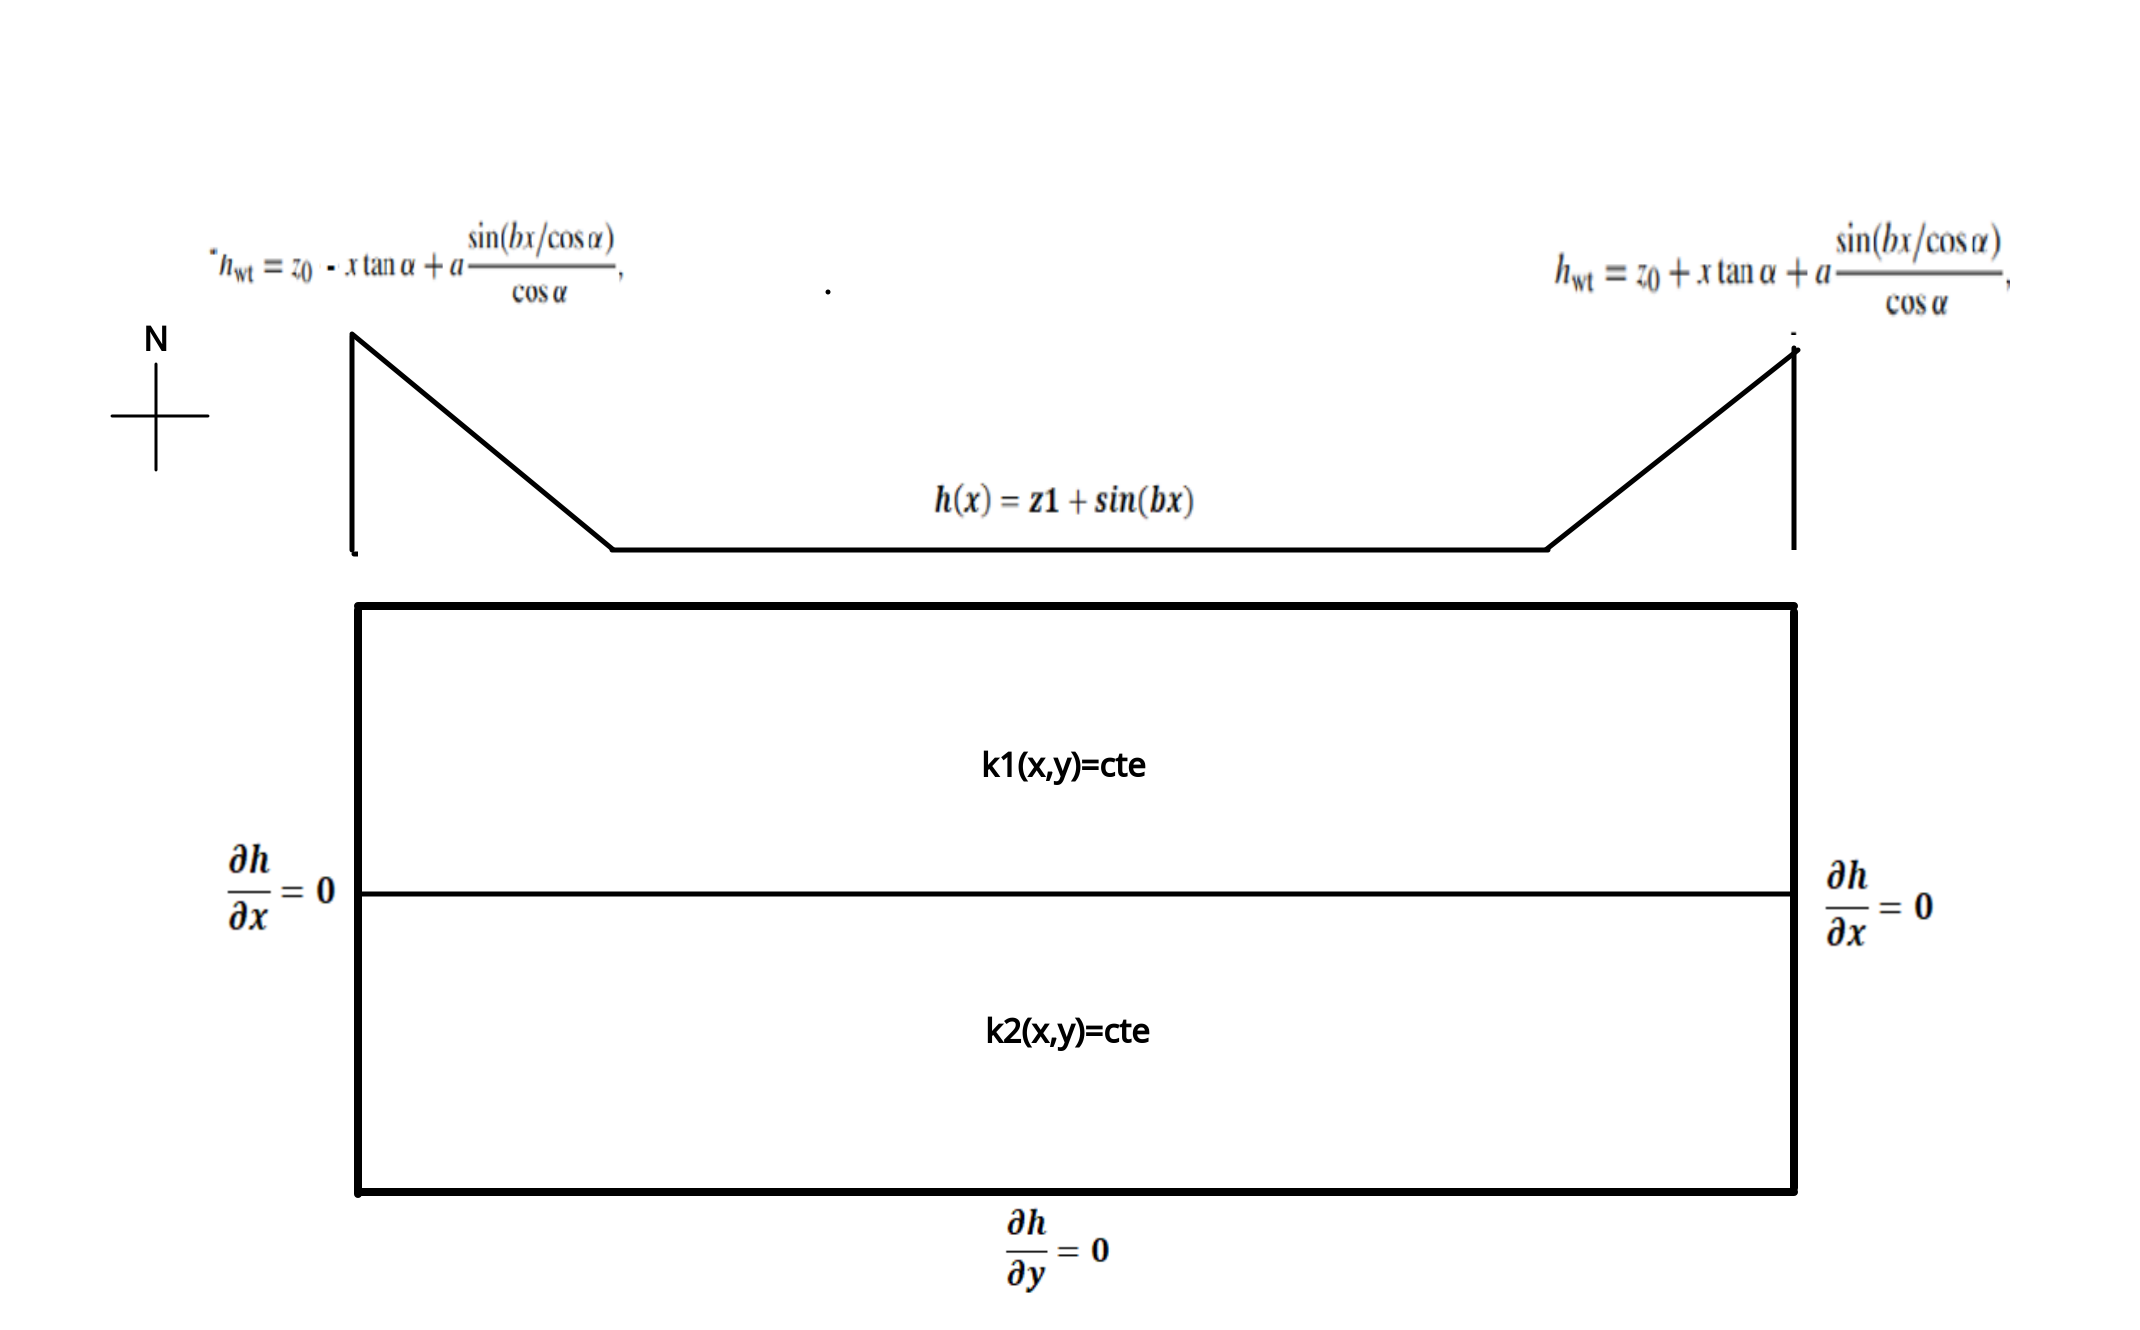
\includegraphics[scale=0.22]{Figura_29b.png}
\caption{ Modelo matemático conceptual}
\label{Figura3:7a}
\end{figure}

\begin{figure}[h]
\centering
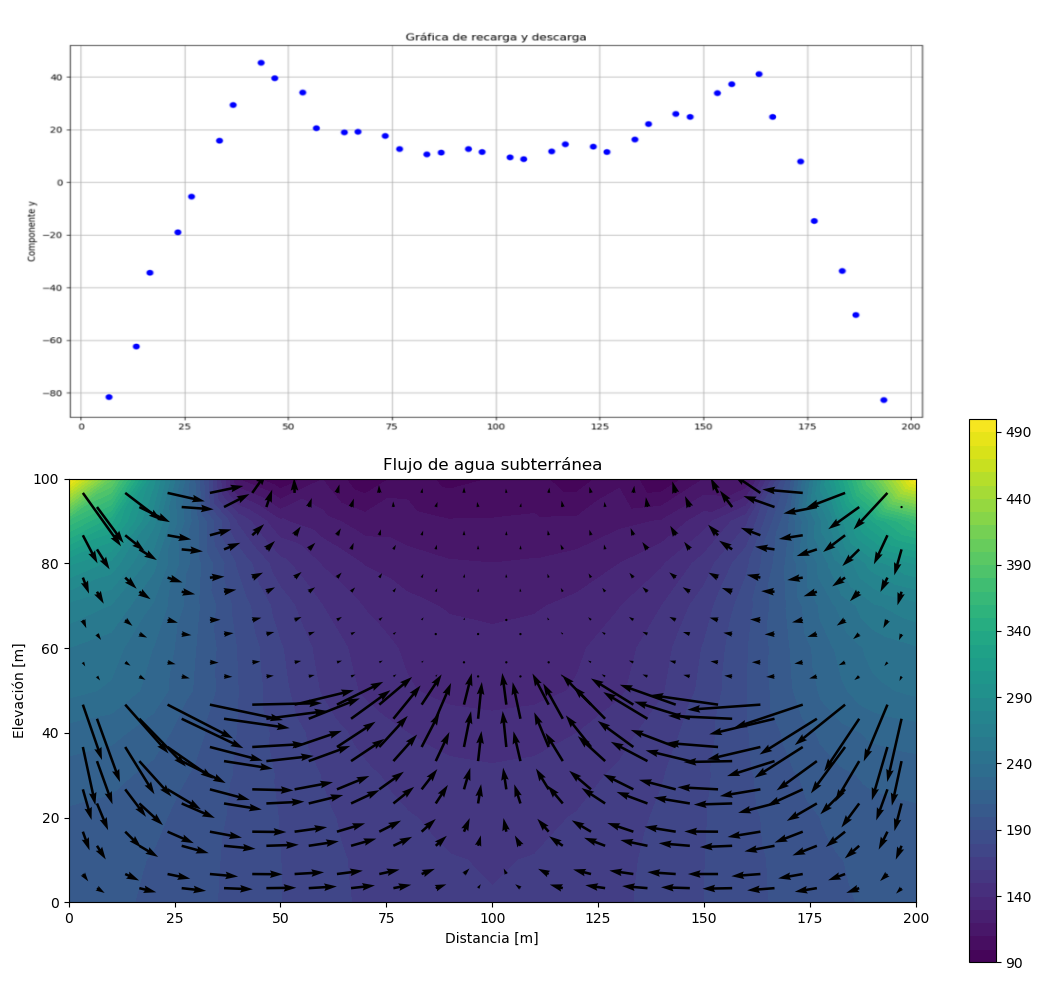
\includegraphics[scale=0.55]{Figura_35d.png}
\caption{ Estratificación grano fino a grueso}
\label{Figura3:7}
\end{figure}
 
\begin{figure}[H]
\centering
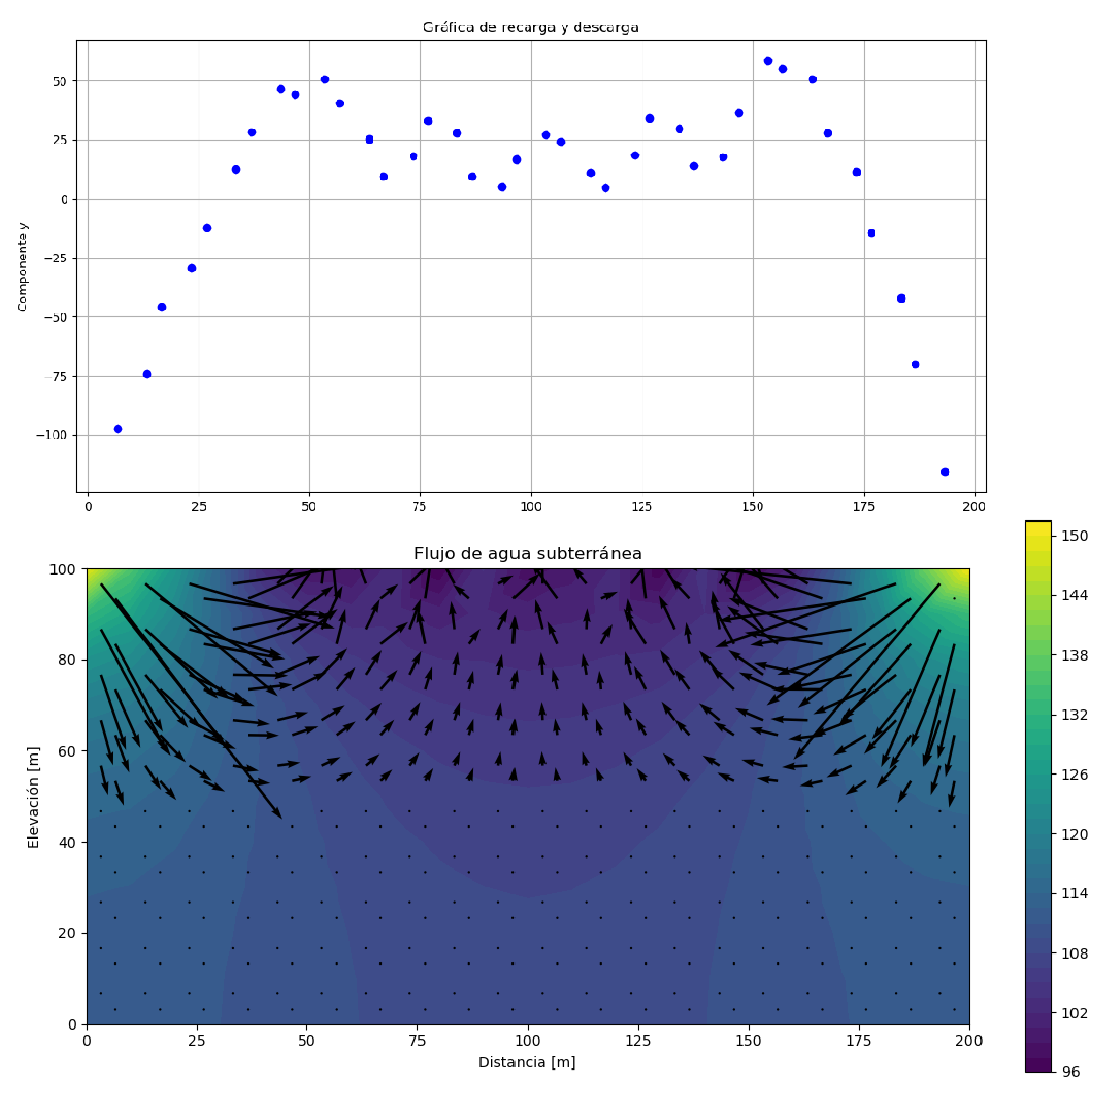
\includegraphics[scale=0.55]{Figura_36d.png}
\caption{ Estratificación grano grueso a fino}
\label{Figura3:8}
\end{figure}


Deacuerdo al análisis de la simulación anterior para condiciones de Dirichlet simples. El flujo al momento de atravesar un material con una conductividad hidráulica más alta provoca una deformación en las isolíneas de carga hidráulica, por lo que el flujo atraviesa rapidamente el material y de la misma forma asciende hacie el centro del valle; en el caso del estrato de menor conductividad en la zona inferior del modelo (figura \ref{Figura3:8}), las lineas de flujo son incapaces de penetrar la capa impermeable y las lineas de flujo ascienden de forma casi vertical en el centro del valle.

\section{Caso heterogéneo aleatorio}

En las simulaciones anteriores, la conductividad hidráulica se asignaba según el modelo geológico propuesto y a partir de este se determinaban los patrones de flujo y las zonas de almacenamiento, sin embargo, según lo escrito en la sección 1.2.1,  en realidad la conductividad dentro de una formación de una misma composición, varia según la distribución de una variable aleatoria, es decir, la conductividad se distribuye según una función de distribución en cada punto, lo que llamaremos heterogeneidad aleatoria. Para este caso, donde las simulaciones estan determinadas en cada punto del dominio por una función aleatoria $K(\textbf{x})$, la ecuación que modela el problema es el siguiente:

 \begin{equation}
\label{eqn:mys19}                         
\dfrac{\partial}{\partial{x}}(K(\textbf{x})\dfrac{\partial{h}}{\partial{x}})+\dfrac{\partial}{\partial{z}}(K(\textbf{x})\dfrac{\partial{h}}{\partial{z}})=0
\end{equation}

Donde la función aleatoria K(\textbf{x}) representa su variación espacial y esta caracterizada por un semivariograma teórico $\gamma(h)$. 

\subsection{Simulación 5: Condiciones de frontera simples}

El modelo conceptual-teórico consiste en el estudio de una zona con material poroso cuya composición varia según una distribución de probabilidad, donde el movimiento del flujo se realiza de forma similar que el modelo estudiado en las simulaciones homogéneas. La simulación se realiza en un material de la misma composición pero con tratamiento de la conductividad heterogénea para determinar las caracteristicas del flujo y el campo de cargas hidráulicas. 
\\

La ecuación diferencial que modela el problema es la misma que en el caso homogéneo (ecuación \ref{eqn:mys3}), de igual forma se ocuparan las mismas condiciones de frontera (ecuación \ref{eqn:mys4}, \ref{eqn:mys4a} y \ref{eqn:mys5}). La diferencia principal en este modelo es la definición de los subdominios para cada conductividad hidráulica, donde cada elemento finito resulta ser un subdominio en la que se hará una asignación de cada realización de la función aleatoria $K(\textbf{x})$.

 \begin{equation}
\label{eqn:mys20}                         
{\Omega}={\Omega}_{1}{\cup}{\Omega}_{2}...{\Omega}_{i}..{\Omega}_{n} 
\end{equation} 

 \begin{equation}
\label{eqn:mys21}                         
{\Omega}_{i}=T_{i}(l)
\end{equation}

Donde n es el número de elementos finitos del espacio de discretización $\hat{H}_{1}$
. En la ecuación \ref{eqn:mys20} cada subdominio es representado por el elemento finito $T_{i}$ que se delimita por las coordenadas de los grados de libertad $l$. La formulación variacional se realiza de la misma forma que en el caso heterogéneo simple, fraccionando la forma bilineal en $n$ planteamientos para cada elemento.

\begin{equation}
 \label{eqn:mys22}
 a(h,v)=\int_{\Omega_{1}}^{} k_{1}{\nabla}h{\cdot}{\nabla}v \cdot ds+\int_{\Omega_{2}}^{} k_{2}{\nabla}h{\cdot}{\nabla}v \cdot ds+...+\int_{\Omega_{i}}^{} k_{i}{\nabla}h{\cdot}{\nabla}v \cdot ds+...+\int_{\Omega_{n}}^{} k_{n}{\nabla}h{\cdot}{\nabla}v \cdot ds
\end{equation}

Para obtener los valores de la función aleatoria $K(\textbf{x})$, se realizará un promedio de 4 simulaciones no condicionales sobre la malla de los centroides (vease sección 2.4.2) para ser asignados en cada elemento. El semivariograma teórico que se ocupó de caracterizar la función aleatoria será un semivariograma exponencial (ecuación 2.1.1) con rango=15, sill=1 y nugget=0. Para la resolución del problema se ocupará el espacio de discretización $\hat{H}_{1}$ definida en la ecuación \ref{eqn:mys8}, mientras que para la definición de la heterogeneidad en cada elemento se ocupará un espacio de funciones $H^{2}$ correspondiente a los elementos de Lagrange discontinuos. Los resultados se muestran a continuación:

\newpage


\begin{figure}[H]
\centering
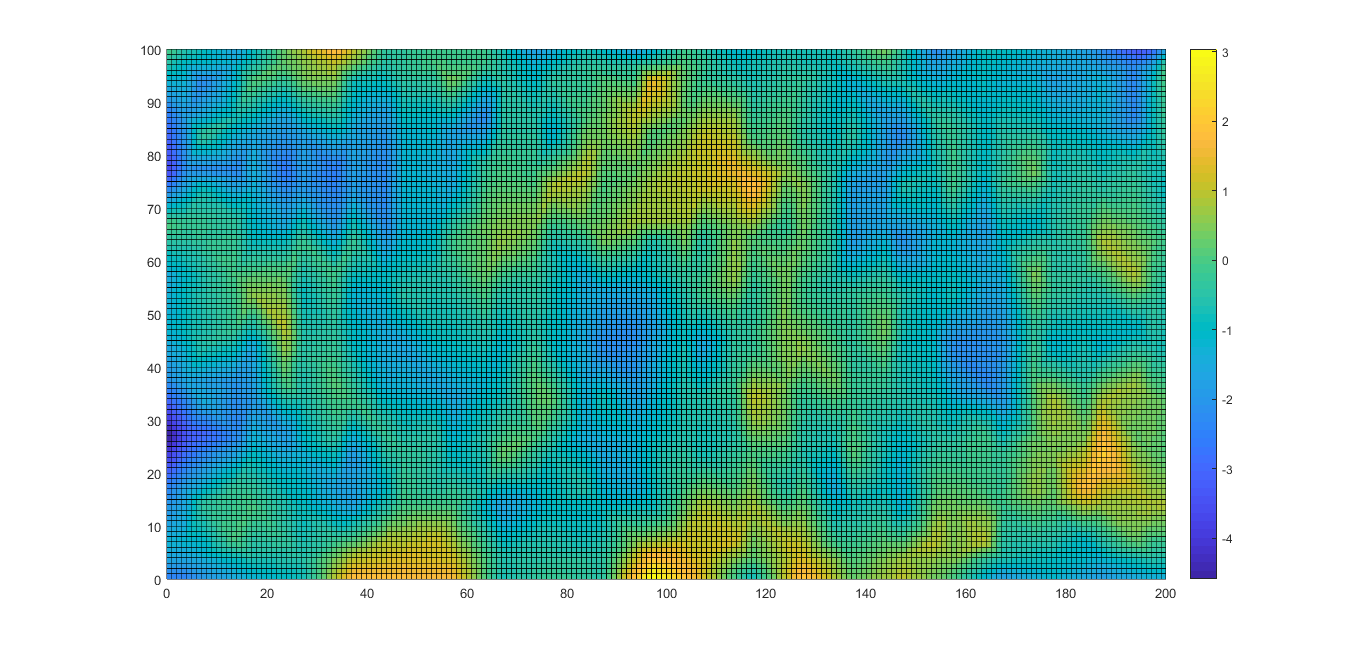
\includegraphics[scale=0.45]{Figura_37.1.png}
\caption{ Disribución de conductividad hidráulica logaritmica resultado de la simulación no condicional ln(K)}
\label{Figura3:9.1}
\end{figure}

 \begin{figure}[H]
\centering
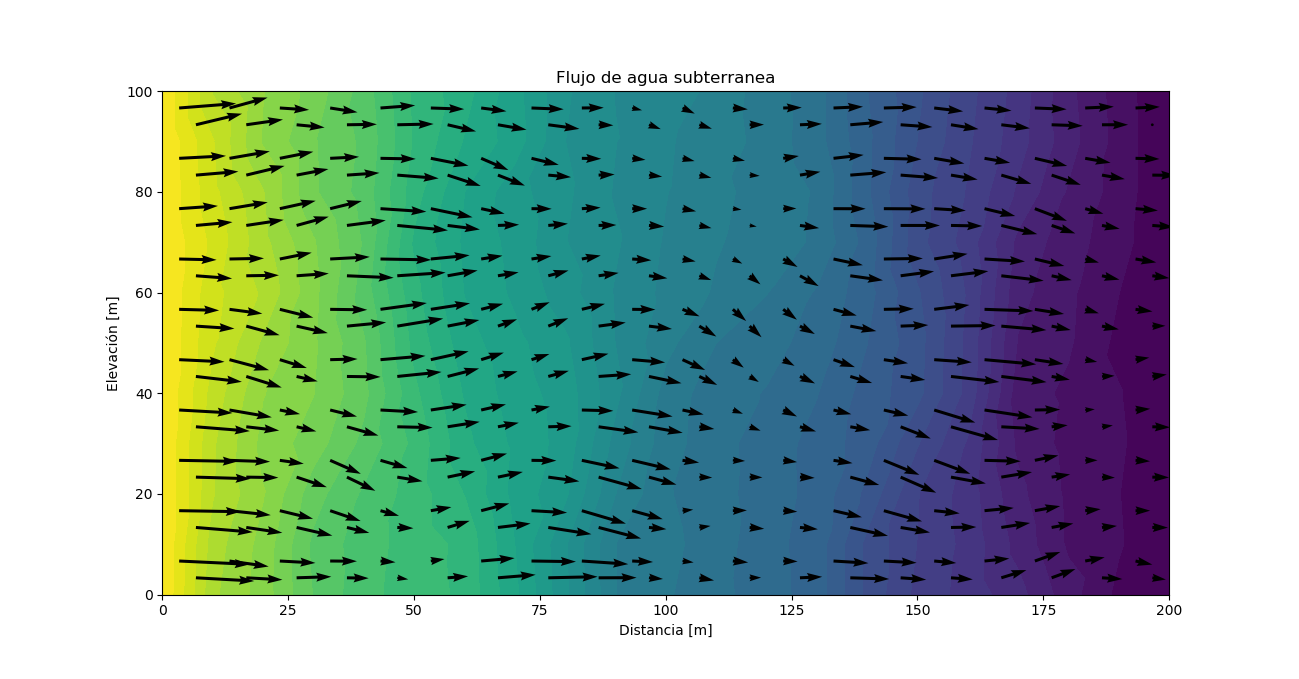
\includegraphics[scale=0.50]{Figure_37.png}
\caption{ Campo de cargas hidráulicas y flujo para un medio poroso heterogéneo aleatorio isótropo}
\label{Figura3:9}
\end{figure}

\newpage


En la figura \ref{Figura3:9.1} podemos observar las estructuras que aparecen en el medio, resultado de una simulación no condicional; mientras que en la figura \ref{Figura3:9} podemos observar como a diferencia de la simulación en un material homogéneo mostrada en la figura \ref{Figura20:2}, las lineas de flujo se ven modificadas según la posición en la que se encuentran debido a la variación de la conductividad del material. En ocasiones estas lineas de flujo convergen en ciertas zonas y siguen su camino hacia la frontera de baja carga hidráulica, otras buscan salir por la frontera impermeable, pero ninguna tiene una preferencia de dirección.
\\

La anterior simulación considera que la conductividad se comporta de forma isotrópa en todo el dominio; por lo que para abarcar un concepto más amplio de heterogeneidad, se realizaron dos simulaciónes bajo las mismas condiciones anteriores pero considerando un medio donde la conductividad es anisótropa; para ello, se definio un elipse de anisotropía, donde el eje mayor se define en la dirección preferencial de la conductividad hidráulica y su caracterización se realiza partir de un semivariograma teórico, mientras que el eje menor se define a partir de una proporción del semivariograma definido en la dirección preferencial. 
\\

Los elipses de anisotropía se definieron en su dirección máxima con el semivariograma del ejemplo isótropo (rango=15, sill=1 y nugget=0) y con una proporción de 0.1 en la dirección de menor preferencia; para la primer simulación, el eje mayor fue en dirección norte, mientras que para la segunda simulación, el eje mayor fue en dirección este.

\begin{figure}[H]
\centering
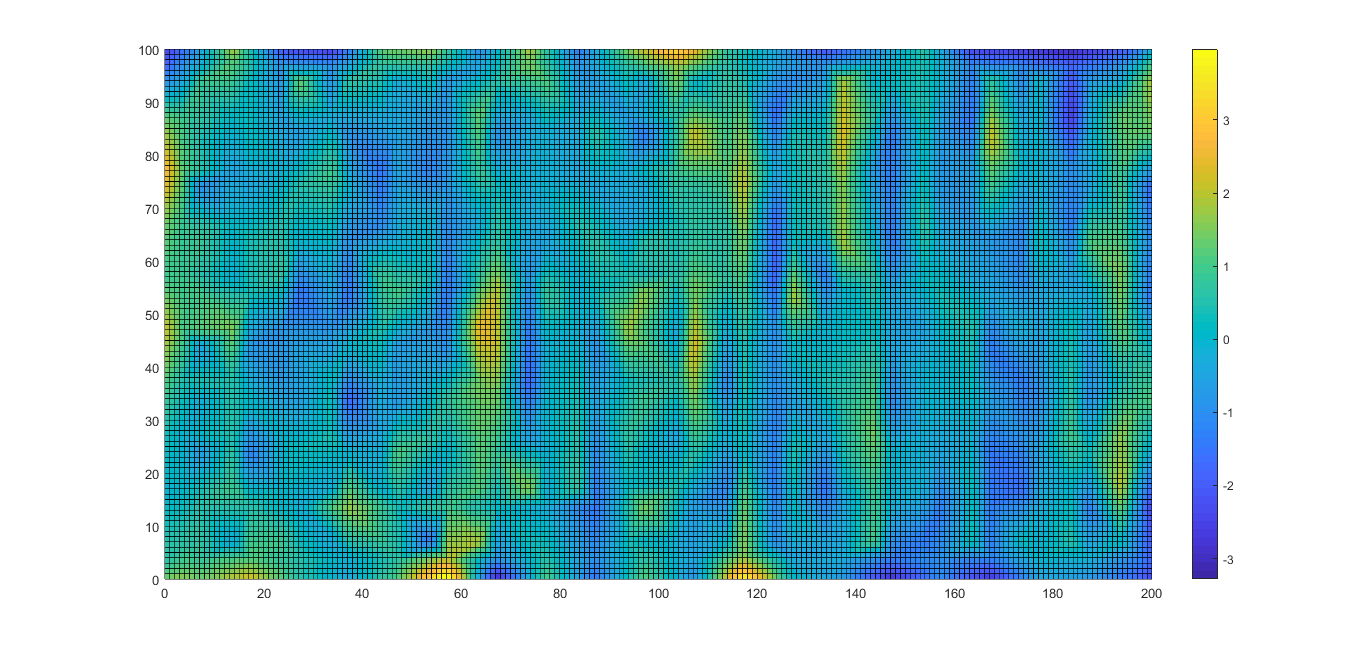
\includegraphics[scale=0.45]{Figura38}
\caption{ Distribución de la conductividad hidráulica logaritmica ln(K) para un medio anisótropo con dirección prefencial Norte }
\label{Figura3:10}
\end{figure}

 \begin{figure}[H]
\centering
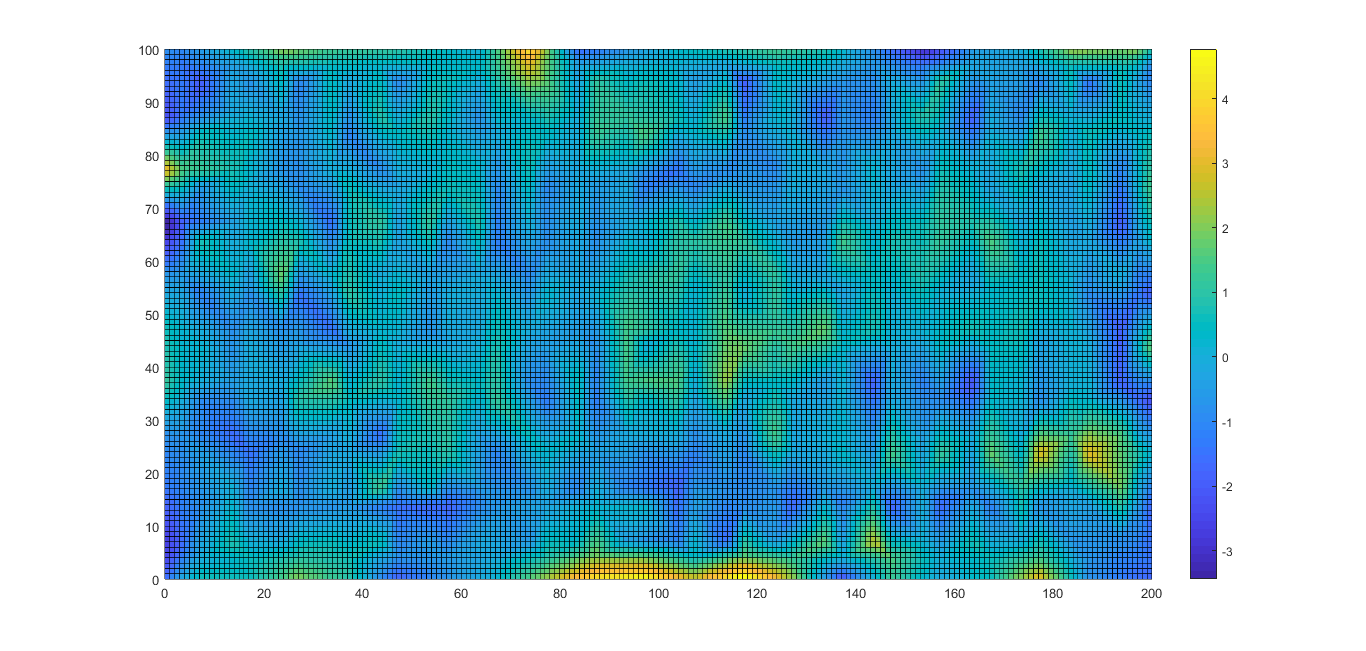
\includegraphics[scale=0.45]{Figura39}
\caption{ Distribución de la conductividad hidráulica logaritmica ln(K) para un medio anisótropo con dirección prefencial Este }
\label{Figura3:11}
\end{figure} 

Como se puede observar en las figuras \ref{Figura3:10} y \ref{Figura3:11}, a diferencia de las estructuras resultantes de una simulación no condicional en un medio isótropo (Figura \ref{Figura3:9.1}), estas aparecen alargadas en su dirección preferencial, por lo que la dirección que toma el flujo cambiaria según la forma de la estructura.

\begin{figure}[H]
\centering
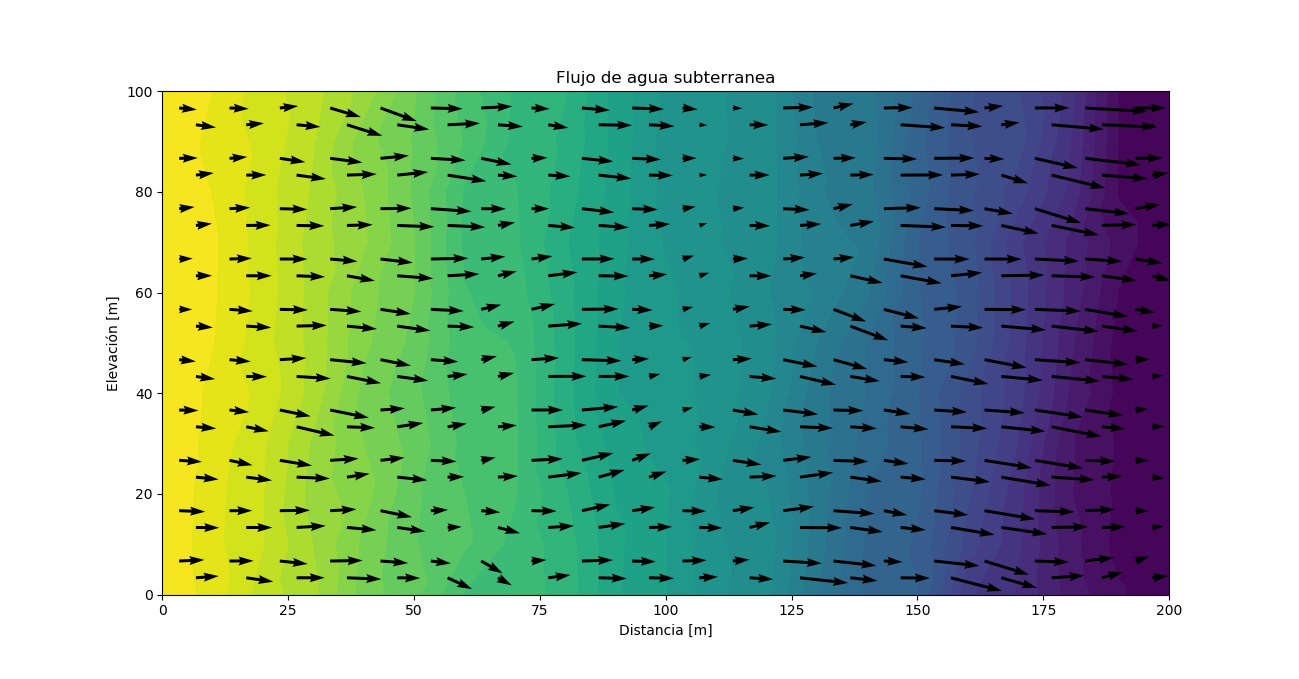
\includegraphics[scale=0.50]{Figura_40}
\caption{ Campo de cargas hidráulicas y flujo para un medio poroso heterogéneo aleatorio anisótropo (Dirección norte) }
\label{Figura3:10}
\end{figure}

 \begin{figure}[H]
\centering
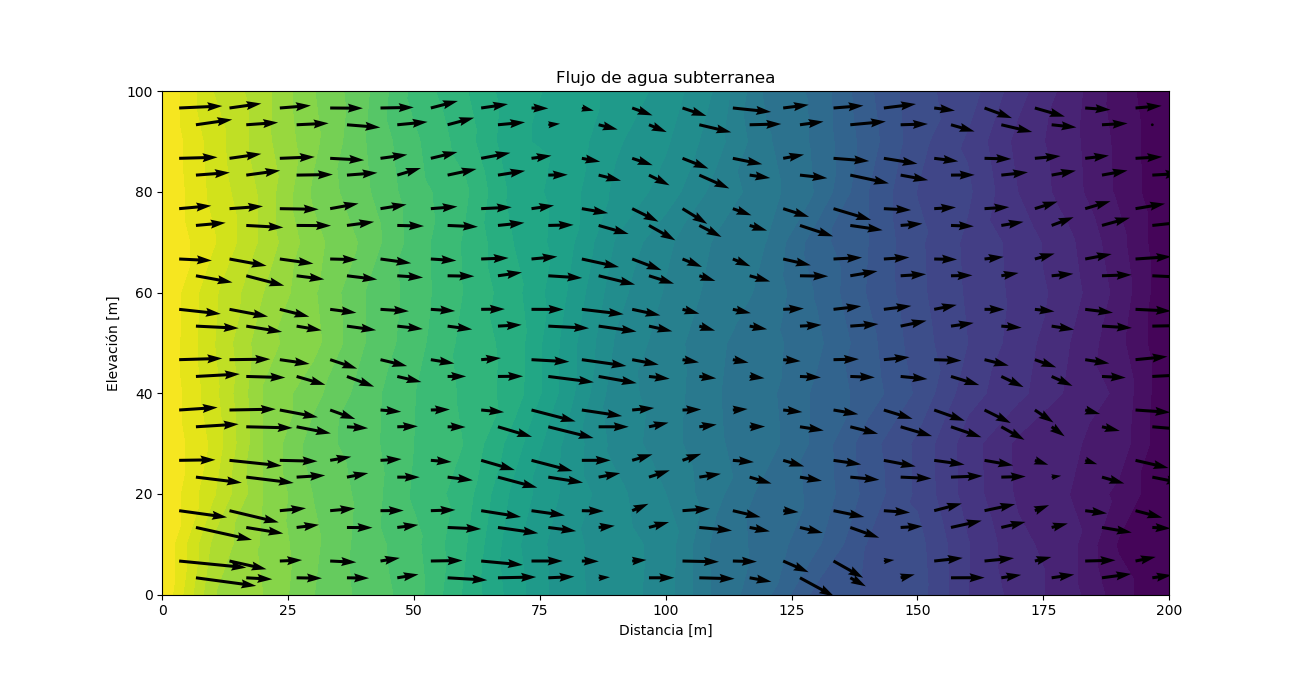
\includegraphics[scale=0.50]{Figura_41}
\caption{ Campo de cargas hidráulicas y flujo para un medio poroso heterogéneo aleatorio anisótropo (Dirección este) }
\label{Figura3:11}
\end{figure} 

A diferencia de los resultados mostrados para un medio isótropo (Figura \ref{Figura3:9}), se puede observar como las lineas de flujo rodean las estructuras con formas más alargadas según su dirección preferencial. 
 
\newpage
